% Plantilla realizada por Gonzalo Matarrubia. Basada en la plantilla creada por
% Alberto Brunete (UPM) que, a su vez está basada en la de Santiago Morante Cendrero (UC3M)

%parametros de tipo libro
\documentclass[10pt,a4paper]{book}

%idioma español y acentos
\usepackage[spanish, es-tabla]{babel}
\selectlanguage{spanish}
\usepackage[utf8]{inputenc}
\usepackage[fixlanguage]{babelbib}
\selectbiblanguage{spanish}

%algunos símbolos matemáticos y paquete para usar subimágenes
\usepackage{amsmath}
\usepackage{amsfonts}
\usepackage{amssymb}
\usepackage{graphicx}
\usepackage{subfigure}
\usepackage{listings}
\usepackage{appendix}
\usepackage{eurosym}
\usepackage{fancyhdr}
\usepackage{float}
%\usepackage{natbib}
%Márgenes
\usepackage[left=3cm,top=3cm,right=3cm,bottom=3cm]{geometry}

%
\usepackage{multicol}

%para generar Índice con hipervínculos
\usepackage{hyperref}
\usepackage[style=index , nonumberlist, toc]{glossaries}

%Algunas variables recurentes
\def\TFM{Entorno de desarrollo y testing para una aplicacion Flutter en un sistema embebido
 basado en Yocto proyect}
\def\ME{Gonzalo Matarrubia González}
\def\TUTOR{Borja Bordel Sánchez}
\def\MASTERNAME{Máster Universitario en Software de Sistemas Distribuidos y Empotrados}
\def\DATE{Junio 2022}

%parametros del documento (sus propiedades)
\hypersetup{
    pdftitle={Entorno de desarrollo y testing para una aplicacion Flutter en un sistema embebido basado en Yocto proyect - TFM - 2022},
    pdfsubject={TFM - 2022},
    pdfauthor={Gonzalo Matarrubia González},
    pdfkeywords={Yocto} {Yocto Project} {Qemu} {Raspberry pi} {Flutter} {embedded} {development enviroment},
    colorlinks,
    citecolor=black,
    filecolor=black,
    linkcolor=black,
    urlcolor=blue,
}

% Estableciendo estilos para el código C/C++, Consola y Python
\usepackage{xcolor}
\definecolor{codegreen}{rgb}{0,0.6,0}
\definecolor{gray97}{gray}{.97}
\definecolor{gray91}{gray}{.91}
\definecolor{gray75}{gray}{.75}
\definecolor{gray45}{gray}{.45}
\definecolor{codegray}{rgb}{0.5,0.5,0.5}
\definecolor{codepurple}{rgb}{0.58,0,0.82}
\definecolor{backcolour}{rgb}{0.95,0.95,0.92}

\lstset{ frame=Ltb,
	framerule=0pt,
	aboveskip=0.5cm,
	framextopmargin=3pt,
	framexbottommargin=3pt,
	framexleftmargin=0.2cm,
	framesep=0pt,
	rulesep=.4pt,
	backgroundcolor=\color{gray97},
	rulesepcolor=\color{black},
	%
	stringstyle=\ttfamily,
	showstringspaces = false,
	basicstyle=\small\ttfamily,
	commentstyle=\color{gray45},
	keywordstyle=\bfseries,
	%
	numbers=left,
	numbersep=15pt,
	numberstyle=\tiny,
	numberfirstline = false,
	breaklines=true,
}
\lstnewenvironment{listing}[1][]
{\lstset{#1}\pagebreak[0]}{\pagebreak[0]}

\lstdefinestyle{consola}
{
	basicstyle=\small\ttfamily,
	backgroundcolor=\color{gray91},
	commentstyle=\color{gray45},
    keywordstyle=\color{magenta},
    numberstyle=\tiny\color{codegray},
    stringstyle=\color{codepurple},
	language=bash,
}

\lstdefinestyle{C}
{
	language=C,
}
\lstdefinestyle{Flutter}
{
	language=Flutter,
}

%Definimos el segundo nivel de listas como guiones
\renewcommand{\labelitemii}{-}
%Definimos estilo de página para el documento
\pagestyle{fancy}
\fancyhf{}
\renewcommand{\headrulewidth}{0pt}
%\rhead{\thesection }
\cfoot{\thepage}

%Glosario
%Índice de términos y abreviaturas
\makeglossaries % create makeindex files
%\newacronym{NAME}{NAME}{Description}
\newacronym{SDK}{SDK}{Software Development Kit}
\newacronym{OS}{OS}{sistema operativo}
\newacronym{UI/UX}{UI/UX}{interfaz y experiencia de usuario}
\newacronym{QA}{QA}{asegurador de calidad}
\newacronym{WSL}{WSL}{Windows subsystem for Linux}
\newacronym{WSL2}{WSL2}{Windows subsystem for Linux version 2}
\newacronym{FPGAs}{FPGAs}{Dispositivos lógicos programables basado en \emph{arrays} de puertas lógicas}
\newacronym{ADT}{ADT}{kit de desarrollo de aplicaciones}
\newacronym{IoT}{IoT}{internet de la cosas}
\newacronym{SBC}{SBC}{computadoras de una sola placa, normalmente el tamaño de una tarjeta
bancaria. Suelen ser dispositivos de bajo consumo y de propósito específico}
\newacronym{rpi}{rpi}{Raspberry Pi}
\newacronym{IDE}{IDE}{entorno de desarrollo integrado}
\newacronym{Code}{Code}{Visual Studio Code}
\newacronym{vscode}{vscode}{Visual Studio Code}
\newacronym{cross-compile}{cross-compile}{compilación cruzada}
\newacronym{IaaC}{IaaC}{infrasturure as a code}
\newacronym{OTA}{OTA}{over the air}
\newacronym{MVP}{MVP}{producto mínimo viable}
\newacronym{API}{API}{interfaz de programación de aplication}

%\newglossaryentry{sample}{name={sample}, description={an example}}
\newglossaryentry{bootloader}{name={bootloader},description={Programa de gestión de arranque}}
\newglossaryentry{hipervisor}{name={hipervisor},description={Programa que añade una capa de virtualización
entre el sistema operativo y el microprocesador, se utiliza común mente para ejecutar más de una aplicación
o sistema operativo en un sólo microprocesador, de forma tal que ambas parte piensen que tiene el uso
exclusivo del micro}}
\newglossaryentry{KVM}{name={KVM},description={Módulo del kernel de linux que permite a éste actuar como un hipervisor}}
\newglossaryentry{XEN}{name={XEN},description={hipervisor de tipo 1 desarrollado originalmente por
la Universidad de Cambridge y posteriormente mantenido por la Linux Fundation}}
\newglossaryentry{Linux Foundation}{name={Linux Foundation},description={Es un consorcio tecnológico
sin ánimo de lucro establecido para adoptar el crecimiento de Linux}}
\newglossaryentry{startup}{name={startup},description={Empresa de nueva creación con posibilidad
de un gran crecimiento gracias a la comercialización de productos o servicios de tecnologías
de la información y comunicación}}
\newglossaryentry{SDLC}{name={SDLC},description={ciclo de vida de desarrollo de software,
por sus siglas en inglés}}
\newglossaryentry{Raspberri Pi}{name={Raspberry Pi},description={Popular SBC de bajo coste}}
\newglossaryentry{DevOps}{name={DevOps},description={Es la cultura empresarial que busca una colaboración
más estrecha entre los equipos de desarrollo y operaciones}}
\newglossaryentry{Widgets}{name={Widgets},description={Aplicativo o componente de la interfad
que realiza una función específica}}
\newglossaryentry{compilacion cruzada}{name={compilación cruzada},description={Es aquella compilación
que tiene como objetivo la ejecución del código en una computadora con una arquitectura diferente
a la computadora utilizada para la compilación}}
\newglossaryentry{front-end}{name={front-end},description={En una aquitectura software basada
en capas, nos referimos a las capas que conformen la interfaz como fron-end}}
\newglossaryentry{back-end}{name={back-end},description={En una aquitectura software basada
en capas, nos referimos a las capas de servicios o con la lógica del programa como back-end}}
\newglossaryentry{scripts}{name={scripts},description={Pequeño conjunto de instrucciones
que permite automatizar una tarea repetitiva}}
\newglossaryentry{shell}{name={shell},description={Consola de sistema}}
\newglossaryentry{framework}{name={framework},description={Es un gran conjunto de librerías que
proveen de un gran número de recursos de desarrollo.}}
\newglossaryentry{CI/CD}{name={CI/CD},description={Integración y entrega continua. Por
sus siglas en inglés.}}
\newglossaryentry{on premises}{name={on premises},description={Hace referencia a cuando
un servidor CI/CD es propiedad de la empresa, a nivel hardware, y por tanto no está externalizado
en cloud.}}
\newglossaryentry{git}{name={git},description={Herramienta de control de versiones}}
\newglossaryentry{plugins}{name={plugins},description={Módulo software que añade una funcionalidad
específica y adicional a un programa}}
\newglossaryentry{pipeline}{name={pipeline},description={Documento de texto en lenguaje de marcado
que describe las características de la infraestructura de CI/CD, así como las pruebas o
procesos que sufre el código en dicha infraestructura}}
\newglossaryentry{open source}{name={open source}, description={Es una corriente de software
que aboga por la publicación del código fuente para poder ser mantenido por la comunidad de usuarios}}
\newglossaryentry{fetch}{name={fetch},description={Acto de descarga del código fuente de un repositorio}}
\newglossaryentry{on-premises}{name={on-premises},description={Estrategia de infraestructura
software que cuando se tiene el hardware en propiedad de la propia empresa}}
\newglossaryentry{coding standard}{name={coding standard},description={Documento formal
que suelen tener las empresas en el que se describe las reglas de estilo con las que
se pogramará en cada lenguaje. Todos los desarrolladores deben cumplir estas reglas para
que haya uniformidad}}
\newglossaryentry{early bird}{name={early bird},description={Un comprador que aceptaría participar en
un programa de beta-testing con tal de acceder al producto de manera anticipada}}
\newglossaryentry{ports}{name={ports},description={Se llama ports a aplicaciones que fueron
desarrolladas para un sistema y que en vez de volver a desarrollarse de nuevo para otro
sistema usan alguna técnica de adaptación del código}}

\glsaddall


%empieza el documento
\begin{document}
%elementos antes del trabajo en sé se meten dentro de frontmatter
\frontmatter

%cada incluye referencia a un archivo de tipo .tex
\begin{titlepage}
\begin{center}

%forma de introducir imágenes. el \\[0.5 cm] de final de línea introduce un salto de ese tamaño.
%width=1\textwidth indica el tamaño de la imágen (valores entre 0-1).
\begin{flushleft}
 
\includegraphics[width=0.35\linewidth]{imgs/logo-etsisi.png}  \\[0.5 cm]
\end{flushleft}

\LARGE \MASTERNAME \\ [1 cm]

\Huge \textsc{\TFM}\\[1 cm]

\LARGE \textbf{PROYECTO FIN DE MASTER}\\[1 cm]

\LARGE \ME \\[1 cm]

%flushleft alinea a la izquierda el texto

\LARGE

%rellena de blanco el resto de la p�gina para escribir abajo del todo
\vfill

% Bottom of the page
{\large \DATE}

\end{center}
\end{titlepage}
\begin{titlepage}
\begin{center}

%forma de introducir imgenes. el \\[0.5 cm] de final de lnea introduce un salto de ese tamao.
%width=1\textwidth indica el tamao de la imgen (valores entre 0-1).
\begin{flushleft}
    
\includegraphics[width=0.35\linewidth]{imgs/logo-etsisi.png}  \\[0.5 cm]
\end{flushleft}

\LARGE \MASTERNAME \\ [1 cm]

\LARGE \textbf{TRABAJO FIN DE MASTER}\\[1 cm]

\Huge \textsc{\TFM} \\[1 cm]


\hfill \break
\hfill \break

\begin{multicols}{2}
\begin{flushleft}
\Large \emph{Firma Autor}
\end{flushleft}

\begin{flushright}
\Large \emph{Firma Tutor}
\end{flushright}

\end{multicols}

%rellena de blanco el resto de la página para escribir abajo del todo
\vfill

\end{center}
\end{titlepage}
%Licencia opcional
\begin{flushleft}

Copyright \copyright 2022. Gonzalo Matarrubia González

%ejemplo de licencia, se puede elegir cualquier otra

\paragraph{} Esta obra est licenciada bajo la licencia
Creative Commons Atribución-NoComercial-SinDerivadas 3.0 Unported (CC BY-NC-ND 3.0).
Para ver una copia de esta licencia, visite http://creativecommons.org/licenses/by-nc-nd/3.0/deed.es
o enve una carta a Creative Commons, 444 Castro Street, Suite 900, Mountain View, California,
 94041, EE.UU.

\paragraph{} Todas las opiniones aquí expresadas son del autor, y no reflejan necesariamente las opiniones
de la Universidad Politécnica de Madrid.

\end{flushleft}
\cleardoublepage

\begin{flushleft} \large
\textbf{Título:} \TFM \\
\textbf{Autor:} \ME \\
\textbf{Tutor:} \TUTOR \\

\end{flushleft}

\hfill \break
\begin{center} \LARGE
EL TRIBUNAL \\ [1 cm]
\end{center}

\begin{flushleft} \LARGE
Presidente: \\ [1 cm]
Vocal: \\ [1 cm]
Secretario: \\ [1.5 cm]
\end{flushleft}

\large
Realizado el acto de defensa y lectura del Trabajo Fin de Máster el día
 ....... de ....................   de ... en .........., en la Escuela Técnica Superior
 de Ingeniera y Sistemas Informáticos de la Politécnica de Madrid, acuerda otorgarle la
 CALIFICACIÓN de: \\ [2 cm]

\begin{center}
 \large VOCAL \\ [2.2 cm]
\end{center}

\begin{minipage}{0.5\textwidth}
 \begin{flushleft}
 \large SECRETARIO
\end{flushleft}
\end{minipage}
\begin{minipage}{0.5\textwidth}
\begin{flushright}
 \large PRESIDENTE
\end{flushright}
\end{minipage}


%las referencias a artículos se ponen con \cite,
%las referencias a glosario \gls,
%y las referencias a ecuaciones \eqref
%las referencias a imgenes, tablas o figuras o secciones
% se ponen con \ref (sólo número) o con \hyperref[sec:X]{text}
\chapter{Agradecimientos.}\label{sec:agradecimientos}

\paragraph{}Quiero agradecer el apollo a mi familia: mi padre Manuel, mi madre Reme y mi hermano Álvaro.
También estoy muy agradecido a mi chica Alejandra, ella me animó a dar el paso definitivo para hacer este
máster. \\
Quiero agradecer a todos los profesores que se supieron adaptar a la perfección a una situación
pandémica que obligó sin aviso a dar las clases online. Su profesionalidad y entrega hizo que no
se perdiesen clases ni se quedaran contenidos sin dar. \\
Por último, agrader a mi tutor \TUTOR, al que contacté con una idea de TFM en mente y decidió
aceptarla desde el primer momento.

A todos, gracias de corazón.


\begin{flushright}
G. Matarrubia
\end{flushright}

%
\vspace*{\fill}

\emph{""¡No me importa si funciona en tu máquina! ¡No estamos vendiendo tu máquina!".}

\begin{flushright}
	Vidiu Platon
\end{flushright}

\vspace*{\fill}
%

\cleardoublepage
%chapter introduce un nuevo capítulo
\chapter{Resumen.}

\paragraph{}Este trabajo pretende recoger los aspectos de diseño e implementación
tenidos en cuenta para la creación de un entorno de desarrollo, bajo unos requisitos
tecnológicos y empresariales específicos. Explicará cómo debe ser usado por los
desarrolladores, teniendo en cuenta el ciclo de vida de desarrollo de software (SDLC,
por sus siglas en inglés). Además, se presenta el desarrollo software de una aplicación
de meteorología en un dispositivo embebido Raspberry Pi, que servirá de ejemplo de
los procesos descritos.

\paragraph{}Los requisitos tecnológicos marcados, representan una situación ficticia
que podría darse en una nueva empresa de rápido crecimiento o \textit{start up} dedicada
al ámbito del IoT o sistemas embebidos. Los requisitos son los siguientes:
pequeña empresa en rápido crecimiento, equipo multidisciplinar, se quiere un entorno
flexible y dínamico accesible para adaptarse a rápidamente a cambios de hardware y
a las decisiones empresariales y estratégicas de operaciones. Además se quiere basar
el proyecto en tecnologías que permitan esta rápida adaptación, que sean herramientas
de uso universal, en la medida de lo posible, y de código abierto.

\paragraph{Palabras clave:} Entornos de desarrollo, Yocto, Flutter, sistemas embebidos,
 Raspberry Pi, Qemu, IoT, SDLC.

\chapter{Abstract}

\paragraph{}This document aims to talk about the design and implementation aspects in
the creation of an development environment with some technological and business requirements.
It explains how it should be used by developers in their journy, taking in consideration
the software development life cyle(SDLC). Also, It shows the development of an
metherological application for an embedded device. In this case, a Raspberry Pi. It
is used as example for the process showed previously.

\paragraph{} The technological requirements are the following: A start up in the field
of IoT or embeded devices wants and development environment. It has to be for a fast-growing
and multidisciplinary team. It must be flexible enough for adapting to the business
and strategical choices. It should be universal and open source code based, as much as
it could be possible.

\paragraph{Key words:} IDE, Development environment, Yocto Project, Flutter, embedded
systems, Raspberry Pi, Qemu, IoT, SDLC.

%las referencias a artículos se ponen con \cite,
%las referencias a glosario \gls,
%y las referencias a ecuaciones \eqref
%las referencias a imgenes, tablas o figuras o secciones
% se ponen con \ref (sólo número) o con \hyperref[sec:X]{Blabla}


%genera índice
\tableofcontents

%Índice de figs.
\listoffigures

%Índice de tablas.
\listoftables

%Glosario
\printglossaries % input files created by makeindex

%empieza la parte descriptiva del trabajo
\mainmatter
\chapter{Introducción.}\label{sec:introduccion}

%En este capítulo no deben faltar los siguientes apartados:


\section{Motivación del proyecto}

\paragraph{}Hace un año presenté una idea en un concurso de creación de empresas. Mi
idea de empresa estaba basada en el campo de los dispositivos embebidos o IoT. Fue
entonces cuando empecé ha pensar en los desafios tecnológicos que podrían conllevar la
creación de dicha empresa y cómo, estos desafios debían de estar alineados con los
aspectos de negocio.

\paragraph{}Las \glsplural{startup} no siguen las mismas reglas que las empresas tradicionales.
Ésto es debido a que suelen ser empresas concevidas por pocos emprendedores con recursos
limitados, que deben enfrentarse continuamente a cambios y manejar un riesgo alto en
sus decisiones. Por tanto, si una \gls{startup} es de ámbito tecnológico, dicha tecnología tiene
que estar orientada a ser universal y flexible.

\hfill \break

\begin{figure}[ht]
    \centering
    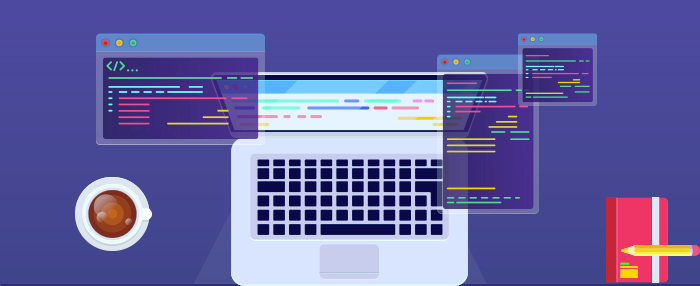
\includegraphics[width=0.65\textwidth]{imgs/dev-env.jpg}
    \caption{Entorno de desarrollo.}
    \label{fig:dev-env}
\end{figure}

\hfill \break

\section{Objetivos}

\paragraph{} Los objetivos de este proyecto se pueden categorizar en objetivos principales,
lo cuales son considerados como esenciales para  definir el éxito del proyecto y
objetivos secundarios que sin ser esenciales nos permiten complementar el análisis,
aprender y sacar conclusiosiones adicionales igualmente valiosas. En conjunto podemos
definir, los siguiente objetivos:

\begin{itemize}
	\item Objetivos Principales
	\begin{itemize}
		\item Diseño e implementación del entorno de desarrollo.
		\item Diseño e implementación del ciclo de vida del desarrollo software.
		\item Explicación del uso del entorno de desarrollo según los roles del equipo
		de desarrolladores.
		\item Diseño e implementación del software de sistema.
		\item Diseño e implementación de una aplicación de meteorología (frontend y backend)
		de características básicas.
		\item Procesos de \textit{testing} y \textit{deployment} de software manuales.
	\end{itemize}
	\item Objetivos Secundarios
	\begin{itemize}
		\item Análisis y justificación de las decisiones tomadas.
		\item Uso de herramientas de código abierto.
		\item Ampliación en las características demostradas con la aplicación de
		meteorología.
		\item Procesos de \textit{testing} y \textit{deployment} de software automátizados.
	\end{itemize}
\end{itemize}


\section{Materiales utilizados}

\paragraph{}Los elementos necesarios para este proyecto son:

\begin{itemize}
	\item Un ordenador de desarrollo.
	\item Ordenador, máquina virtual o servidor de control de versiones.
	\item Ordenador, máquina virtual o servidor de compilaciones.
	\item Una Raspberry Pi conectada a la red local de los desarrolladores.
	\item Pantalla y cable de alimentación de la Raspberry Pi.
\end{itemize}

\section{Estructura del documento}

\paragraph{}A continuación y para facilitar la lectura del documento, se detalla el
contenido de cada capítulo.

\begin{itemize}
\item En el capítulo \ref{sec:introduccion} se realiza una introducción.
\item En el capítulo \ref{sec:estadodelarte} se hace un repaso al estado actual de las
soluciones existentes para abordar las premisas de este proyecto.
\item En el captíulo \ref{sec:EscenarioTrabajo} se presenta al equipo ficticio de
desarrollo, se habla de sus necesidades y de cómo van a interactuar con el entorno.
\item En el capítulo \ref{sec:ManualDeInstalacion} se detallan las instruciones para la
instalación y puesta en marcha del entorno de desarrollo en cada sistema operativo.
\item En el capítulo \ref{sec:GuiaDeUso} se explica las principales herramientas y
opciones presentes en el entorno de desarrollo.
\item En el capítulo \ref{sec:AplicacionMeteorologica} se detallan los aspectos teóricos
de la aplicación de meteorología tales como su interfaz, requisitos y arquitectura.
\item En el capítulo \ref{sec:Desarrollo} se conecta los apartados teóricos de \ref{sec:GuiaDeUso}
y \ref{sec:AplicacionMeteorologica} con la aplicación práctica de los mismos.
\item En el capítulo \ref{sec:cicd} se analíza el ciclo de vida del desarrollo software
y la infraestructura necesaria para llevarlo a cabo.
%\item En el capítulo \ref{sec:}
\item En el capítulo \ref{sec:resultados} se muestran los resultados del proyecto y se
hace un valoración de los mismos.
\item En el capítulo \ref{sec:gestion} se habla de los diferentes recursos utilizados
así como la planificación del proyecto.
\item En el capítulo \ref{sec:conclusiones} se hace una reflexión personal sobre todo
lo relacionado con el proyecto y los aprendizajes extraídos.
\end{itemize}

%las referencias a artículos se ponen con \cite,
%las referencias a glosario \gls,
%y las referencias a ecuaciones \eqref
%las referencias a imgenes, tablas o figuras o secciones
% se ponen con \ref (sólo número) o con \hyperref[sec:X]{text}

\chapter{Estado del arte.}\label{sec:estadodelarte}

\paragraph{}En este capítulo se va a tratar el estado actual de las tecnologías
más relevantes para llevar a cabo entornos de desarrollo replicables, flexibles y universales.
Explicaremos qué aspectos son los más interesantes en cada caso y cómo podrían aplicarse.

\section{Yocto Project.}\label{sec:yocto}

\paragraph{} \emph{Yocto Project} es un proyecto colaborativo y de código abierto
de la \emph{Linux Foundation} cuyo objetivo principal es el de producir herramientas y
procesos que permitan crear distribuciones embebidas de sistemas operativos basados
en el Kernel de Linux. Su código está pensado para que las herramientas y las distribuciones
generadas sean agnósticas respecto de la arquitectura del microprocesador así como del
resto del hardware.
\cite{yoctoprojectpage}

\begin{figure}[h]
	\centering
	
\includegraphics[width=0.35\linewidth]{imgs/yocto-logo}
	\caption[Logo Yocto Project]{Yocto Project. Un proyecto de la Linux Fundation}
	\label{fig:yocto_logo}
\end{figure}

\paragraph{} Yocto es, por tanto, una excelente herramienta para asegurar la repetibilidad
de los sistemas, así como para garantizar la seguridad de los mismos, además de ser
flexible y parametrizable. Decimos que es bueno para asegurar la repetibilidad
ya que la empresa toma posesión del sistema operativo entero y deja de depender de
distribuciones de terceros que puedan introducir cambios sin previo aviso. Garantiza la
seguridad ya que tiene un gran soporte de la comunidad \emph{\gls{open source}} cercana
al desarrollo del propio kernel de Linux, proporcionando rápidamente los últimos parches
de seguridad que se publican. Es flexible ya que permite adaptar cualquier cambio
introducido en el hardware, manteniendo antiguas versiones o incluso desarrollar más de
un hardware al mismo tiempo. Esto es un gran ventaja en los tiempos en los que los equipos
de software deben empezar su código sin tener un sistema hardware final, donde incluso
se desarrolle parte del hardware en dispositivos basados en \emph{\gls{FPGAs}} o en
hardware simulado.

\paragraph{} Este proyecto fue fundado en 2010 con el apoyo de grandes multinacionales
y organizaciones. Destaca la estrecha colaboración con \emph{OpenEmbedded}, tomando de
ellos la mayor parte del \emph{OpenEmbedded Project} y su motor de generación (\emph{build
engine}), \textbf{bitbake}.

\paragraph{} Como parte del proyecto, con cada versión de Yocto, se presenta una versión
de Poky. Poky, es una distribuición de referencia, a partir de la cuál, se realizan las
modificaciones para la construción de una distribución propia.

\begin{figure}[h]
	\centering
	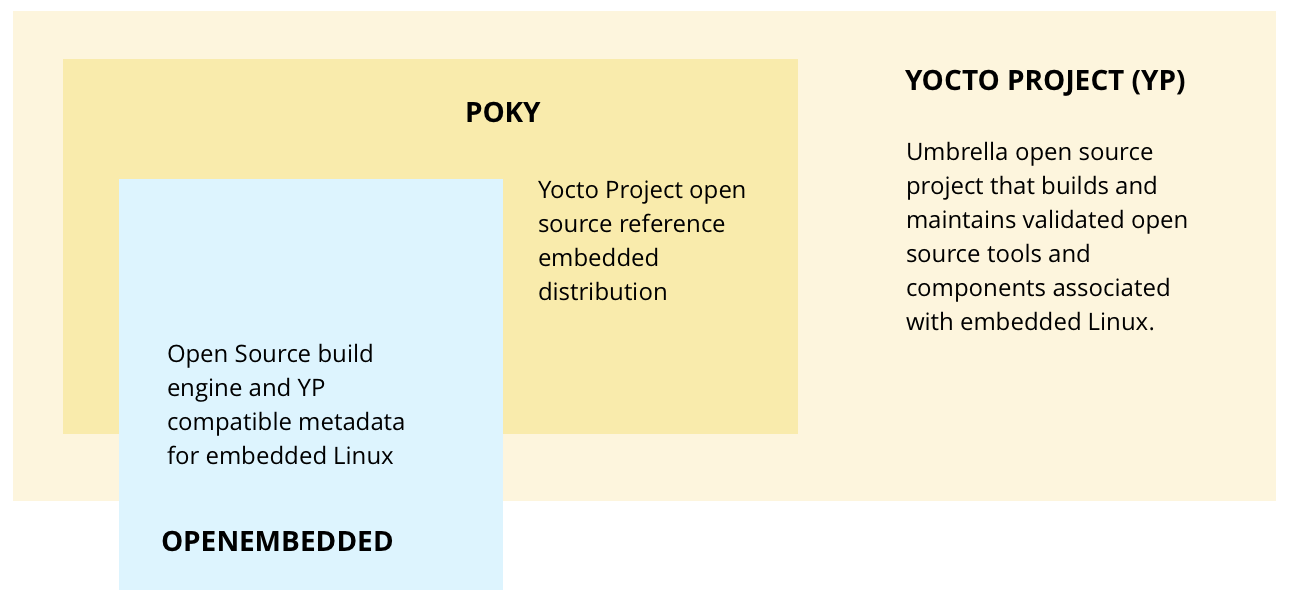
\includegraphics[width=0.60\linewidth]{figs/yocto-overview}
	\caption[Yocto Overview]{Esquema de relación entre Yocto, Poky y OpenEmbedded.}
	\label{fig:yocto_overview}
\end{figure}

\paragraph{}Al principio, Yocto puede resultar ser conceptualmente difícil de entender
ya que su campo de aplicación puede ser muy variado. En este sentido, puede usarse tanto para
la creación de imágenes completas de sistema, creación de \emph{\glsplural{bootloader}}, generación
de sistemas de ficheros (\emph{rootfs}), desarrollo de aplicativos, desarrollo de paquetes
de los aplicativos, desarrollo y/o hacking del kernel y generación de  \emph{toolchains},
\glslink{SDK}{SDKs} o \glslink{ADT}{ADTs}.

\paragraph{\label{layers} \label{recipes}}Los principales conceptos para enterder el
funcionamiento de Yocto, son;
las capas o \emph{layers}, las recetas o \emph{recipes}, las clases y los ficheros de
configuración. Las \emph{recipes} son un conjunto de instrucciones y configuraciones
usadas para la construcción de un paquete. Por ejemplo, una recipe describe la fuente
del código, los parámetros, el compilador y los parches a aplicar así como la instalación
del paquete en la imagen. Las \emph{layers} son conjuntos de recipes agrupadas por
funciones lógicas que interactúan de manera independiente o con una dependencia bien
documentada. Los ficheros de configuración suelen definir un conjunto de variables
dependientes del entorno que queramos construir. Por último, las clases son partes de
código común entre recetas pensadas para ser reutilizadas.

\paragraph{}En cuanto a las opciones de testing, Yocto dispone de test en tiempo
de compilación así como la posibilidad de arrancar las imágenes generadas en una máquina
virtual QEMU \ref{sec:qemu}.

\subsection{Kas.}\label{sec:kas}

\paragraph{}Kas es una herramienta pensada para configurar proyectos basados en bitbake
de una manera sencilla. Kas proveé un \emph{wrapper} de bitbake con comandos de más alto
nivel. Resuelve las tareas de resolución de dependencias, de configuración y de
generación que usualmente suelen hacerse a mano y dejarse documentadas. Yocto
\ref{sec:yocto} utiliza bitbake como motor de generación, por tanto, Kas puede ser
utilizado en proyectos basados en Yocto.
\cite{kas}

\section{QEMU.}\label{sec:qemu}

\paragraph{}Qemu es un emulador de hardware de código abierto capaz de interoperar con
\gls{KVM} para arrancar máquinas virtuales con un rendimiento casi nativo.
\cite{qemu}

\paragraph{}Qemu dispone de los siguientes modos de funcionamiento:

\begin{itemize}
	\item User-mode emulation.
	\item System emulation.
	\item \gls{KVM} Hosting.
	\item Xen Hosting.
\end{itemize}

\begin{figure}[h]
	\centering
	
\includegraphics[width=0.50\linewidth]{imgs/qemu-logo}
	\caption[Qemu Logo]{Logo de QEMU.}
	\label{fig:qemu}
\end{figure}

\paragraph{} El modo ``User-mode emulation'' permite que una sola aplicación compilada
para una arquitectura diferente a la del resto del sistema arranque mediante la ``traducción''
de instrucciones en tiempo real.

\paragraph{} El modo ``System emulation'' es el más común. Se utiliza para simular una
computadora completa, incluidos sus periféricos. Qemu tiene la capacidad de albergar
sistemas operativos Linux, Solaris, Microsoft Windows, DOS y BSD.

\paragraph{} Los modos ``\gls{KVM}'' y ``\gls{XEN}'' son variaciones del modo ``System
emulation'' en el que se simula más o menos hardware con cada uno de los hipervisores cuyo
nombre coincide con el nombre del modo.

\section{Docker.}\label{sec:docker}

\paragraph{}Docker es una herramienta de gestión de contenedores. Dichos contenedores son
una capa de aislamiento a nivel de aplicación que utilizan los recursos del Kernel de Linux
tales como espacios de nombres. A pesar de que no supone un aislamiento tan fuerte como
el que proporcionan las máquinas virtuales, la principal ventaja de los contenedores es
que son mucho más livianos en cuanto a la necesidad de recursos de memoria, disco y computación.
\cite{docker}

\paragraph{} Docker permite empaquetar aplicaciones y todas sus dependencias, de esta
forma tienen una gran capacidad de portabilidad y flexibilidad con respecto al sistema
operativo dónde se ejecuten.

\begin{figure}[H]
	\centering
	
\includegraphics[width=0.50\linewidth]{imgs/docker-logo}
	\caption[Docker Logo]{Logo de Docker.}
	\label{fig:docker}
\end{figure}

\paragraph{} En nuestro caso, Docker nos va a ayudar a empaquetar todo el entorno de
desarrollo y sus dependencias para que su puesta en marcha sea inmediata, también buscará
evitar la heterogeneidad entre los entornos de desarrollo de los diferentes desarrolladores,
así como tener un control de versiones de las propias dependencias y de las variables
de entorno del sistema.

\section{Flutter.}\label{sec:flutter}

\paragraph{} Flutter es un entorno de desarrollo o \gls{SDK} de aplicaciones. El principal
objetivo de Flutter es facilitar la creación de interfaces de usuario que se adapten a
cualquier pantalla y a cualquier dispositivo. En ese sentido, permite que con un sólo
código fuente común se puedan generar aplicaciones para muchos entornos: Android, iOS,
Linux, Windows, Fucsia, etc.
\cite{flutter}

\paragraph{} Flutter sigue la filosofía de programación basada en objetos, y como está pensado
fundamentalmente para entornos gráficos, todos los objetos en Flutter son \gls{Widgets}.

\begin{figure}[h]
	\centering
	
\includegraphics[width=0.50\linewidth]{imgs/flutter-logo}
	\caption[Flutter Logo]{Logo de Flutter.}
	\label{fig:flutter}
\end{figure}

\paragraph{} Gracias a su capacidad para hacer la \gls{cross-compile} sencilla, resulta
ser increiblemente práctico para su uso en aplicaciones embebidas. Permite el desarrollo
de forma aislada del hardware así como el testing de la aplicación. En el apartado
gráfico destaca la persistencia visual entre la interfaz en entornos de desarrollo y
entornos embebidos.

\paragraph{} Está escrito en el lenguaje de programación Dart \ref{sec:dart} y ha sido
desarrollado por Google.

\subsection{Dart.}\label{sec:dart}

\paragraph{}Dart es un lenguaje de programación orientado a objetos de alto nivel.
Está optimizado para interfaces de usuario y para aumentar la productividad de desarrollo,
ya que permite el ``hot debugging''. Una técnica que posibilita cambiar sólo los objetos cuyo
codigo ha sido actualizado, manteniendo el resto en mitad de una sesión de depuración.
\cite{dart}

\paragraph{}Dart permite compilarse en código máquina para tener un rendimiento similar al
de aplicaciones nativas o traducirse a otros lenguajes considerados nativos en sus campos
como por ejemplo JavaScript para su uso en entornos web. Todo eso lo convierte en un
lenguaje de programación multiparadigma que permite el desarrollo tanto del \gls{front-end}
como del \gls{back-end}.

\begin{figure}[H]
	\centering
	
\includegraphics[width=0.50\linewidth]{imgs/dart-logo}
	\caption[Dart Logo]{Logo de Dart.}
	\label{fig:dart}
\end{figure}

\section{Qt.}\label{sec:Qt}

\paragraph{}Qt es un \gls{framework} the interfaces de usuario muy popular y extendido,
se utiliza, fundamentalmente, en sistemas embebidos de cualquier ámbito, desde impresoras
hasta sistemas de armamento. Esto es así porque dispone de \glsplural{API} en C++ y en
Python y ofrece una gran calidad de recursos gráficos y de herramientas. Por ejemplo,
su \gls{IDE} qtCreator facilita muchísimo el desarrollo, ofrece licencias gratuitas para
programas de código abierto, y está muy bien documentada.

\paragraph{}Hasta hace unos años ha sido el framework rey de los sistemas embebidos, pero
con la reciente llegada de \hyperref[sec:flutter]{Flutter} \ref{sec:flutter} a entornos
de escritorio y distribuciones embebidas, puede suponer un cambio de tendencia.

\begin{figure}[H]
	\centering
	
\includegraphics[width=0.30\linewidth]{imgs/qt}
	\caption[Qt Logo]{Logo de Qt}
	\label{fig:qt}
\end{figure}


\section{React Native.}\label{sec:react}

\paragraph{}React Native es una librería basada en la librería React que a diferencia
de ésta, la compilación genera una aplicación nativa para sistemas iOS o Android. Al
estar desarrollada en JavaScript se está convirtiendo en una de las librerías gráficas
más populares. Además permite crear web apps que pueden correr como servicios en local
y ser visualizadas con la ayuda de un navegador web. Existen adaptaciones mediante las
librerías de \hyperref[sec:Qt]{Qt} \ref{sec:Qt} que pueden llevar estás aplicaciones
gráficas a sistemas Linux. Desde un punto de vista práctico, solo sería recomendable
esta opción para \gls{ports}, ya que al no tener un rendimiento nativo y necesitar
adaptadres estamos malgastando los recursos, los cuales suelen ser escasos en los sistemas
embebidos.

\begin{figure}[H]
	\centering
	
\includegraphics[width=0.30\linewidth]{imgs/react-logo}
	\caption[React Logo]{Logo de React}
	\label{fig:react}
\end{figure}

\section{Vagrant.}\label{sec:vagrant}

\paragraph{}Vagrant es un gestor de máquinas virtuales propiedad de HashiCorp que automatiza
su creación y proporciona una interfaz de alto nivel para su gestión, funciona con máquinas
virtuales de VMWare, VirtualBox, AWS, etc. El propósito fundamental de Vagrant es el de
replicar los entornos de ejecución y de desarrollo de forma automática, y que las pruebas
y el desarrollo sean lo más fieles a los entornos de producción de una manera sencilla.

\paragraph{}Su uso resulta muy similar al de \hyperref[sec:docker]{Docker} \ref{sec:docker}
sólo que en este caso se administran máquinas virtuales en vez de containers. Posiblemente
la popularidad de docker ha hecho que Vagrant haya quedado en segundo plano. Otra razón,
por la que Vagrant no ha terminado de ser muy popular es la dependencia con tecnologías
externas de máquinas virtuales, muchas de ellas con necesidad de licencias comerciales,
así como el uso de hipervisores.

\begin{figure}[H]
	\centering
	
\includegraphics[width=0.50\linewidth]{imgs/vagrant-logo}
	\caption[Vagrant Logo]{Logo de Vagrant}
	\label{fig:vagrant}
\end{figure}

\section{Ansible.}\label{sec:ansible}

\paragraph{}Aunque Ansible es confundido muchas veces con \hyperref[sec:docker]{Docker} \ref{sec:docker}
o con \hyperref[sec:vagrant]{Vagrant} \ref{sec:vagrant} aunque resulta ser una tecnología
totalmente diferente. Ansible es una plataforma de software libre para la administración
de equipos. Permite la administración multi-nodo de forma remota y por lotes. Mediante
un equipo orquestador, se puede automatizar el resto de nodos. Se basa en colecciones
de libros de jugadas o \emph{playbooks}.

\paragraph{}Una de las características principales de Ansible es que no tiene ninguna
dependencia salvo la de Python, la cual es asumible ya que la mayoría
de distribuciones Linux trae Python por defecto.

\paragraph{}En nuestro caso, el entorno de desarrollo traerá los playbooks necesarios
para la instalación de las dependencias. Están escritos en playbooks en vez de en scritps
corrientes para poder integrarse en sistemas remotos de administración fácilmente. Desde
el punto de vista de operaciones, Ansible resulta muy conveniente para pasar la configuración
de los entornos de desarrollo como \gls{IaaC} y por tanto usar control de versiones para
la adminsitración y configuración de equipos. En un entorno empresarial real, estos
playbooks posiblemente estarían en un repositorio distinto y se ejecutarían con permisos
de administrador automáticamente, evitando que el usuario necesite el acceso de superusuario.

\paragraph{}Podríamos comparar Ansible con herramientas de Microsoft de gestión remota,
aunque ésto no supone una barrera para que ansible se integre con herramientas de Microsoft
como \emph{Active Directory}.

\begin{figure}[H]
	\centering
	
\includegraphics[width=0.30\linewidth]{imgs/ansible-logo}
	\caption[Ansible Logo]{Logo de Ansible}
	\label{fig:ansible}
\end{figure}

\section{Visual Studio Code.}\label{sec:vscode}

\paragraph{}Visual Studio Code o VSCode abreviadamente es un \glslink{IDE}{IDE} multiplataforma
de código abierto desarrollado por Microsoft. Es un \glslink{IDE}{IDE} ligero y modular
que permite el desarrollo de software en casi todos los lenguajes de programación mediante
la instalación de \gls{plugins}.

\paragraph{}VSCode se puede personalizar completamente al uso requerido en cada caso,
mediante archivos que añaden funcionalidad al \glslink{IDE}{IDE} en tiempo de ejecución
y dependiendo del proyecto abierto. Por ejemplo, un repositorio de Yocto, podría tener unos
ficheros que definieran las tareas más comunes para la generación de Yocto.

\begin{figure}[H]
	\centering
	
\includegraphics[width=0.30\linewidth]{imgs/vscode-logo}
	\caption[Visual Studio Code]{Logo de Visual Studio Code.}
	\label{fig:vscode-log}
\end{figure}

\paragraph{}En muchas ocasiones Visual Studio Code resulta un programa muy conveniente
para su uso como editor básico de texto, al poder tener disponibles todas las características
avanzadas de edición, propias de los programas de edición de código. En el que además,
tenemos una disposición de ventanas manejable con una o más terminales disponibles.

\paragraph{}Por ejemplo, para el desarrollo de Yocto puede ser utilizado cualquier editor
de texto, desde gedit hasta vim en conjunto con cualquier programa de terminal para lanzar los
comandos y probar nuestros cambios. Sin embargo, tener ambas cosas organizadas en la misma
vista, pudiendo tener un árbol de ficheros y varios ficheros abiertos organizados en pestañas
hace que el desarrollo sea más cómodo.


\begin{figure}[H]
	\centering
	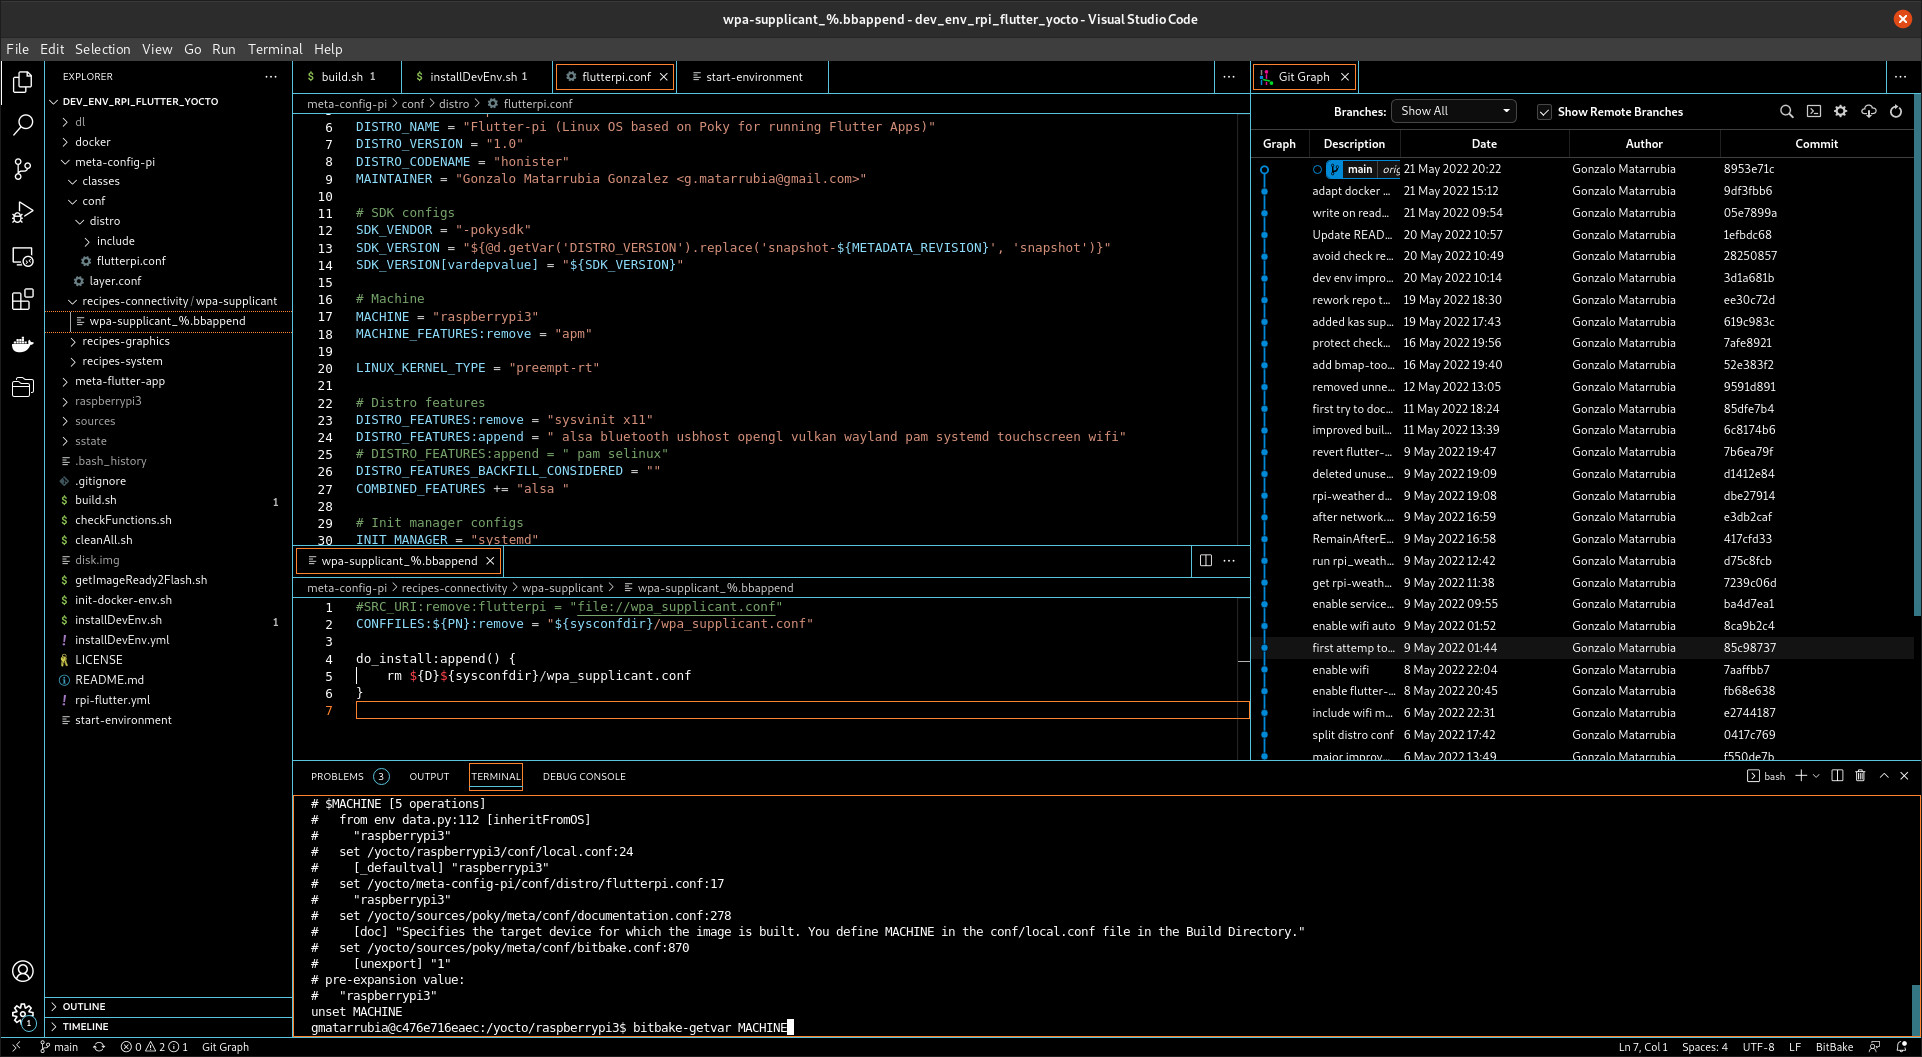
\includegraphics[width=0.90\linewidth]{imgs/vscode-perspective}
	\caption[VSCode yocto]{VSCode usado con Yocto.}
	\label{fig:vscode-perpective}
\end{figure}

\paragraph{}Por su soporte, por su integración con Flutter y todas las razones descritas
anteriormente, hacen de Visual Studio Code el editor perfecto para los entornos de desarrollo
de Flutter y Yocto.

%las referencias a artículos se ponen con \cite,
%las referencias a glosario \gls,
%y las referencias a ecuaciones \eqref
%las referencias a imgenes, tablas o figuras o secciones
% se ponen con \ref (sólo número) o con \hyperref[sec:X]{text}
\chapter{Escenario de trabajo. Descripción y requisitos.}\label{sec:EscenarioTrabajo}

\paragraph{}En este capítulo se presenta al equipo ficticio de desarrollo, se habla
de sus necesidades y de cómo van a interactuar con el entorno. Si consideramos a los
desarrolladores como nuestros clientes o usuarios, podemos aplicar técnicas de análisis
de sus necesidades tales como \textit{Customer Personas} (figura \ref{fig:customer_persona})
o Mapas de Empatía (figura \ref{fig:mapa_empatia}). Estás técnicas son muy comunes
dentro de departamentos de Marketing, su uso garantiza que el diseño del producto se
hará entorno a las necesidades de los clientes, en este caso, del entorno de desarrollo
y los propios desarrolladores. En nuestra versión, vamos a agrupar a los usuarios por
\textit{expertise} y vamos a definir necesidades para equipos.

\begin{figure}[ht]
    \centering
    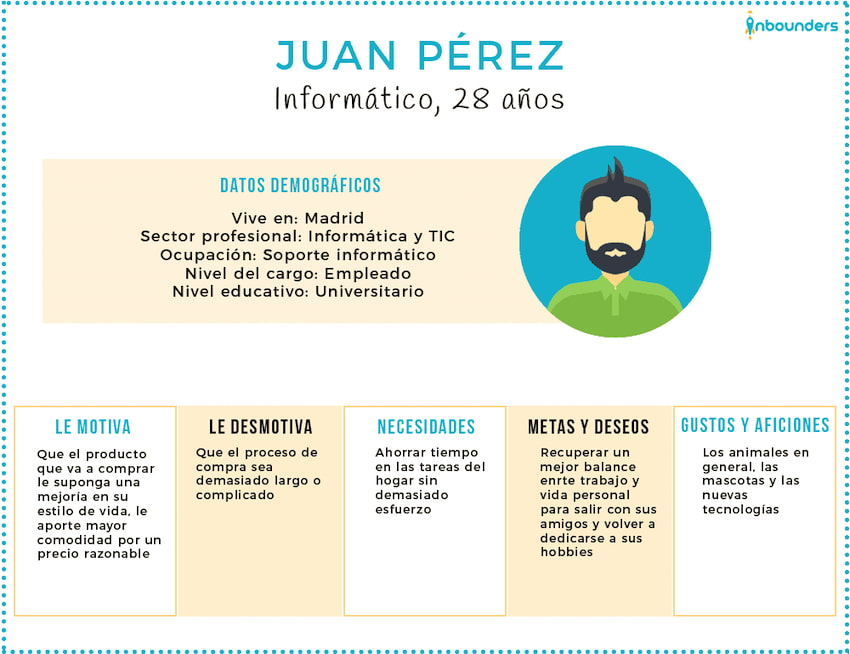
\includegraphics[width=0.65\textwidth]{imgs/buyer-persona-ejemplo.jpg}
    \caption{Ejemplo \textit{Customer Persona} utilizado en Marketing}
    \label{fig:customer_persona}
\end{figure}

\begin{figure}[H]
    \centering
    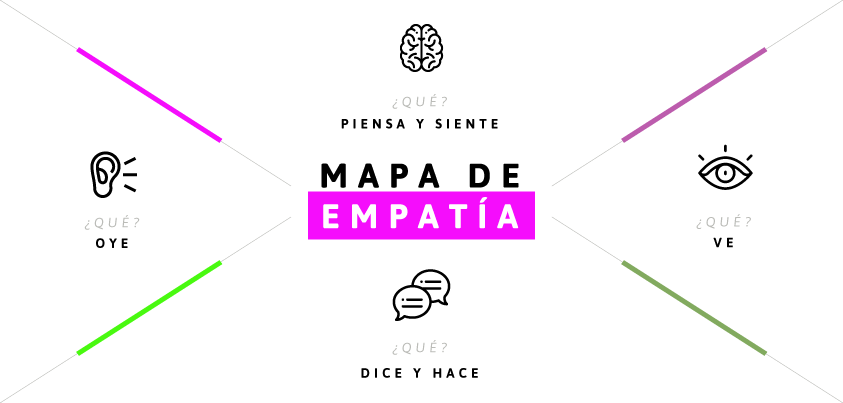
\includegraphics[width=0.65\textwidth]{imgs/mapa-empatia.png}
    \caption{Esquema resumen del Mapa de Empatía utilizado en Marketing}
    \label{fig:mapa_empatia}
\end{figure}

\section{Equipo de desarrollo de software de sistema}

\paragraph{}La gran mayoría de productos de \gls{IoT} basados en microprocesadores,
tienen un sistema operativo sobre el cual se ejecutan las aplicaciones, servicios o
microservicios. Los desarrolladores del software de sistema se encargan de gestionar
este sistema operativo. Los principales aspectos que deben tener en cuenta son:

\begin{itemize}
    \item Proveer de las librerías necesarias para la ejecución de la aplicaciones o
    servicios.
    \item Velar por la estabilidad del sistema.
    \item Asegurar la ciberseguridad del dispositivo.
    \item Proveer el acceso a los recursos hardware por parte del software, mediante
    drivers propios o desarrollados por terceros.
    \item En muchos caso, desarrollan las herramientas de distribuición y despliegue
    de todo el software en los dispositivos.
\end{itemize}

\paragraph{}La principales herramientas de trabajo dentro del entorno de desarrollo para este equipo
será:

\begin{itemize}
    \item Yocto \ref{sec:yocto} y bitbake para el desarrollo de layers \ref{layers} y
    recipes \ref{recipes}.
    \item Uso de la consola o \gls{shell}.
    \item Lenguaje de programación Bash, para el desarrollo de \gls{scripts} que se
    ejecutan en la consola.
    \item Lenguaje de programación Python, para el desarrollo de \gls{scripts} más complejos.
    \item IDE para la edición de todos los ficheros.
\end{itemize}

\section{Equipo de desarrollado de aplicaciones UI/UX}

\paragraph{}Las siglas UI/UX hacen referencia al acrónimo en inglés \emph{User interface
and user experience}, es decir, a la interfaz de usuario y cómo es la interacción con la
misma. Dicho de otra manera, el equipo de UI/UX están a cargo del desarrollo del
\gls{front-end}. Su objetivo es crear una interfaz alineada con las necesidades del
usuario medio al que destinada, así como, generar una experiencia adecuada de uso. Es
importante que la interfaz represente los objetivos de negocio, ya que es la principal
conexión con el usuario y por tanto la mayor fuente de percepción de información y de
imagen de marca.

\paragraph{}Técnicamente, la interfaz debe tener en cuenta las expecificaciones de diseño,
los requisitos, el uso de recursos de cálculo así como los recursos del \gls{SDK}
utilizado para el desarrollo.

\paragraph{}El desarrollo de la interfaz suele ser independiente al desarrollo de la
lógica de los servicios, permitiendo así la autogestión de los equipos de desarrollo.
Sin embargo, para las labores de testing en frecuente necesitar ambas partes para
comprobar que la interfaz se comporta de manera coherente con la lógica. Por eso, el
entorno de desarrollo debe permitir el desarrollo de manera independiente de la interfaz
y la ejecución de ambas maneras, tanto independiente en conjunto con el \gls{back-end}.

\paragraph{}Los principales aspectos que deben tener en cuenta son:

\begin{itemize}
    \item Ejecución independiente de la interfaz.
    \item Ejecución conjunta con el \gls{back-end}.
\end{itemize}

\paragraph{}La principales herramientas de trabajo dentro del entorno de desarrollo para este equipo
será:

\begin{itemize}
    \item IDE.
    \item Lenguaje de programación Flutter/Dart.
\end{itemize}

\section{Equipo de desarrollado de servicios de aplicaciones}

\paragraph{}Blabla

\section{Equipo de integración y distribución DevOps}

\paragraph{}Blabla

\section{Equipo de testing y QA}

\paragraph{}Blabla

%las referencias a artculos se ponen con \cite,
%las referencias a imgenes \ref,
%las referencias a glosario \gls,
%y las referencias a ecuaciones \eqref

\chapter{Manual de Instalación.}\label{sec:ManualDeInstalacion}

\paragraph{}En este capítulo se va a explicar cómo instalar el entorno de desarrollo
para cada uno de los principales sistemas operativos. Los pasos descritos se podrán
seguir con independencia del estado previo del sistema. No se asume ningún estado previo.

\section{Consideraciones previas}

\begin{itemize}
    \item El sistema operativo y sus principales tecnologías y herramientas tienen
    como base su uso en sistemas operativos GNU/Linux, concretamente la versión 20.04 de
    la distribución de Ubuntu. Por lo que, a pesar de poder ser utilizados en cualquier
    sistema, serán en éstos donde será más fácil y óptimo su uso.

    \item Al igual que sucede en otros capítulos de este documento, se van a diferenciar
    las dos partes lógicas que componen el proyecto software: el entorno Flutter y el
    entorno Yocto.

    \item La inicaciones de este capítulo parten de sistemas con instalaciones por defecto
    y sin modificar, actualizados a la última versión disponible. Es posible que algún
    paso pueda variar, se pueda prescindir de algún paso, o que se requiera algún paso
    adicional, en función del tipo de instalación o versión.
\end{itemize}

\section{Instalación del entorno Flutter}\label{sec:entflutter}

\paragraph{}En el entorno Flutter vamos a ser capaces de desarrollar la aplicación,
pasar sus test y compilarla para diferentes plataformas.

\subsection{Instalación en sistemas operativos GNU/Linux}

\paragraph{}Para la instalación de este entorno en un sistema operativo basado en
la versión de Ubuntu 20.04 se podrá optar por tres estrategias: correr el entorno de
forma nativa, utilizar el método basado en docker o utilizar la característica de
desarrollo en container de Visual Studio Code, que sería una solución intermedia.

\subsection{Desarrollo en container de vscode.}

\paragraph{}\textbf{Nota:} Este método podría requerir permisos de \emph{sudo} o super
usuario en caso de que docker no esté previamente instalado.

\begin{enumerate}
    \item Instalar \textbf{\gls{git}} y \textbf{docker} (\emph{sólo si es necesario}).
    \begin{lstlisting}[style=consola, numbers=left]
        $ sudo apt install -y git
    \end{lstlisting}

    \item Clonar el repositorio desde github y entrar en el directorio.
    \begin{lstlisting}[style=consola, numbers=left]
        $ git clone https://github.com/Gmatarrubia/rpi_weather.git
        $ cd rpi_weather
    \end{lstlisting}

    \item Instalar Docker.
    \begin{lstlisting}[style=consola, numbers=left]
        $ source checkFunctions.sh
        $ check_docker
    \end{lstlisting}
    \textbf{Nota:} Después de este paso podría ser necesario reiniciar, la salida del
    script nos indicará si ésto fuera necesario. Si reiniciáramos, abririamos una
    terminal, iríamos al directorio del repositorio y continuaríamos con el siguiente
    paso.

    \item Instalar Visual Studio Code.
    \begin{lstlisting}[style=consola, numbers=left]
        $ source checkFunctions.sh
        $ check_vscode
    \end{lstlisting}

    \item Abrir el repositorio con \gls{vscode}
    \begin{lstlisting}[style=consola, numbers=left]
        $ code .
    \end{lstlisting}

    \item Reabrir la carpeta en el container como nos sugerirá.
    \begin{figure}[H]
        \centering
        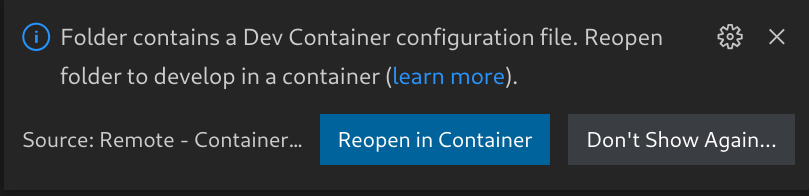
\includegraphics[width=0.55\textwidth]{imgs/dev-container}
        \caption[Mensaje emergente en vscode]{Mensaje emergente en vscode.}
        \label{imgs:vscode-devcontainer}
    \end{figure}

    \item Fin de la instalación. En caso de que no \gls{vscode} no detecte el \gls{SDK}
    reiniciar \gls{vscode} y volver a abrirlo y volver a dar a ``abrir en container''.
\end{enumerate}

\subsection{Entorno de desarrollo dockerizado.}

\paragraph{}\textbf{Nota:} Este método podría requerir permisos de \emph{sudo} o super
usuario en caso de que docker no esté previamente instalado.

\begin{enumerate}
    \item Instalar \textbf{\gls{git}} (\emph{sólo si es necesario}).
    \begin{lstlisting}[style=consola, numbers=left]
        $ sudo apt install -y git
    \end{lstlisting}

    \item Clonar el repositorio desde github
    \begin{lstlisting}[style=consola, numbers=left]
        $ git clone https://github.com/Gmatarrubia/rpi_weather.git
        $ cd rpi_weather
    \end{lstlisting}

    \item (Opcional) En caso de necesitar instalar Visual Studio Code para el desarrollo,
    se puede utilizar la siguente opctión.
    \begin{lstlisting}[style=consola, numbers=left]
        $ source checkFunctions.sh
        $ check_vscode
    \end{lstlisting}

    \item Ejecutar el script inicialización de container. Este script construye la
    imagen en caso de que no haya sido creada previamente.
    \begin{lstlisting}[style=consola, numbers=left]
        $ ./init-docker-env.sh
    \end{lstlisting}
    \textbf{Nota:} Después de este paso podría ser necesario reiniciar, la salida del
    script nos indicará si ésto fuera necesario. Si reiniciamos, sería necesario volver
    a repetir este último paso para que la instalación continue.

    \item Ejecutar el script de obtención de dependencias.
    \begin{lstlisting}[style=consola, numbers=left]
        (docker)$ ./getSources.sh
    \end{lstlisting}

    \item Fin de la instalación.
\end{enumerate}

\begin{figure}[H]
    \centering
    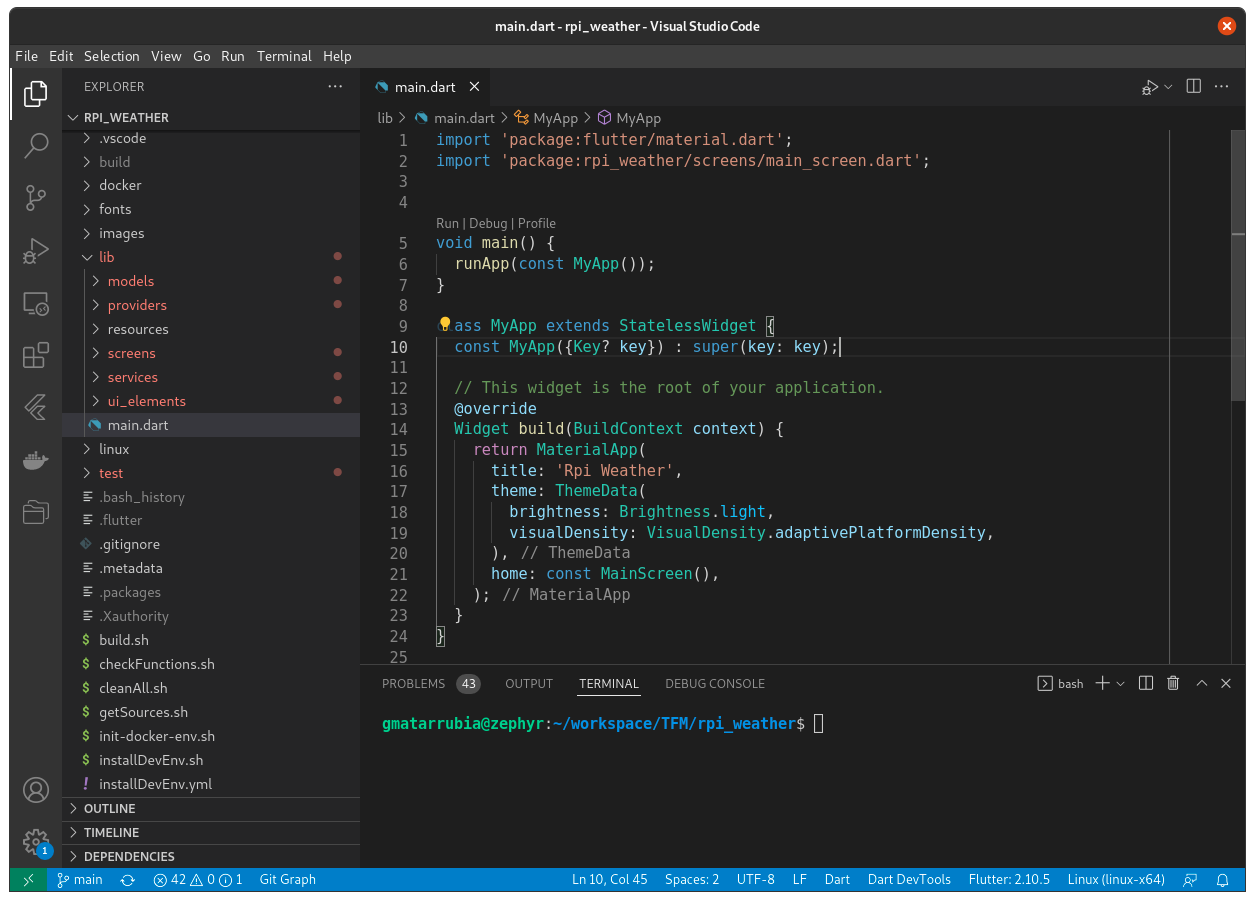
\includegraphics[width=0.95\textwidth]{imgs/vscode-ready}
	\caption[Visual Studio Code]{Visual Studio Code con el proyecto abierto.}
	\label{imgs:vscode-ready}
\end{figure}

\subsection{Instalación nativa.}

\paragraph{}\textbf{Nota:} Este método requiere permisos de \emph{sudo} o super usuario.

\begin{enumerate}
    \item Instalar la herramienta \textbf{\gls{git}} de control de versiones.
    \begin{lstlisting}[style=consola, numbers=left]
        $ sudo apt install -y git
    \end{lstlisting}

    \item Clonar el repositorio desde github
    \begin{lstlisting}[style=consola, numbers=left]
        $ git clone https://github.com/Gmatarrubia/rpi_weather.git
        $ cd rpi_weather
    \end{lstlisting}

    \item Ejecutar el script de instalación de paquetes.
    \begin{lstlisting}[style=consola, numbers=left]
        $ sudo ./installDevEnv.sh
    \end{lstlisting}

    \item Ejecutar el script de obtención de dependencias.
    \begin{lstlisting}[style=consola, numbers=left]
        $ ./getSources.sh
    \end{lstlisting}

    \item (Opcional) En caso de necesitar instalar Visual Studio Code para el desarrollo,
    se puede utilizar la siguente opctión.
    \begin{lstlisting}[style=consola, numbers=left]
        $ source checkFunctions.sh
        $ check_vscode
    \end{lstlisting}

    \item Fin de la instalación.
\end{enumerate}

\subsection{Instalación en sistemas operativos Windows}

\paragraph{}Tanto Visual Studio Code, como el \gls{SDK} de Flutter tienen versiones
nativas para Windows. Aunque en principio, Flutter podría trabajar indistintamente en
versiones Windows y Linux de escritorio, para evitar posibles discrepancias en la
compatibilidad de dependencias se va a trabajar dentro de un entorno Linux llamado
\gls{WSL2}. Esta característica de Windows incluida en la versión 10 y 11 en ambos
casos en la ediciones pro, permite el uso de un sistema operativo basado en el kernel
de Linux dentro del propio sistema Windows sin virtualización del hardware.

\paragraph{}\textbf{Nota:} Se requieren permisos de administrador.

\paragraph{}Por tanto los pasos para obtener nuestro entorno de desarrollo listo para
trabajar son:

\begin{enumerate}
    \item Instalar y configurar \gls{WSL2}. Para ello, abrir una consola, ya sea cmd
    o powershell, con permisos de administrador e introducir el siguiente comando:
    \begin{lstlisting}[style=cmd, numbers=left]
        wsl.exe --install
    \end{lstlisting}

    \item Reiniciar el sistema.

    \item Arrancar \gls{WSL2} desde el Menú de Inicio. Y realizar la configuración
    inicial que se nos indique, normalmente esto consiste en crear un usuario y
    contraseña.

    \item Una vez en la terminal de \gls{WSL2}, comprobamos que todo haya ido bien realizando
    la actualización de los paquetes de sistema con:
    \begin{lstlisting}[style=consola, numbers=left]
        $ sudo apt update
        $ sudo apt upgrade
    \end{lstlisting}

    \item Siguiendo en la terminal de \gls{WSL2}, instalamos la herramienta git y clonamos
    el repositorio.
    \begin{lstlisting}[style=consola, numbers=left]
        $ sudo apt install -y git
        $ git clone https://github.com/Gmatarrubia/rpi_weather.git
    \end{lstlisting}

    \item Instalar Visual Studio Code siguiendo la instalación recomendada en su página
    oficial: \href{https://code.visualstudio.com/download}{https://code.visualstudio.com/download}

    \item Instalar una herramienta de escritorio remoto VNC que soporte tunneling SSH.
    Recomendablemente Gsshvnc, la cual se puede descargar aquí:
    \href{https://github.com/zrax/gsshvnc/releases}{Github Gsshvnc Releases}

    \begin{figure}[H]
        \centering
        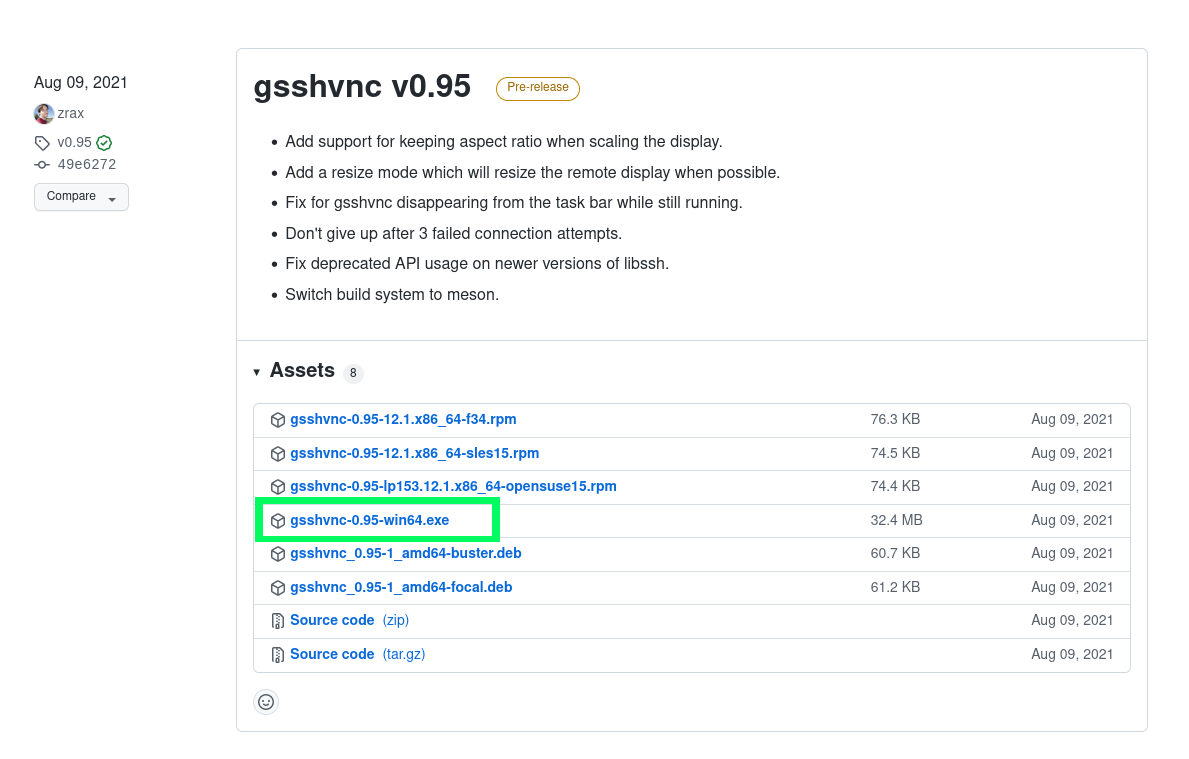
\includegraphics[width=0.95\textwidth]{imgs/gsshvnc-releases}
        \caption[gsshvnc releases]{gsshvnc página de descargas.}
        \label{imgs:gsshvnc-releases}
    \end{figure}

    \item Abrir Visual Studio Code e instalar las extensiones necesarias. Para ello
    una vez en VSCode, utilizar el atajo de teclado \emph{Ctrl+p} e introducir el siguiente
    comando. Debemos aceptar cualquier sugerencia que nos pregunte:
    \begin{lstlisting}[style=cmd]
        ext install ms-vscode-remote.vscode-remote-extensionpack
    \end{lstlisting}

    \item Abrir un entorno \gls{WSL2} en Visual Studio Code y abrir la carpeta del repositorio
    previamente descargado.
    blabla - insertar captura pantalla.

    \item Instalar la extension de Visual Studio Code de Flutter de la misma manera que
    en el paso anterior.
    \begin{lstlisting}[style=cmd]
        ext install Dart-Code.flutter
    \end{lstlisting}

    \item Fin de la instalación.
\end{enumerate}

\subsection{Instalación en sistemas operativos MacOS.}

\paragraph{}Blabla

\newpage
%%%%%%%%%%%%%%%%%%%%%%%%%%%%%%%%%%%%%%%%%%%%%%%%%%%%%%%%%%%%%%%%%%%%%%%%%%%%%%%

\section{Instalación del entorno Yocto}

\subsection{Instalación en sistemas operativos GNU/Linux}

\paragraph{}Al igual que sucedía con el entorno de Flutter \ref{sec:entflutter}, existe
la posibilidad de correr el entorno de manera nativa, de manera \emph{dockerizada} o
mediante el desarrollo en container de \gls{vscode}.
Ambos entornos se han diseñado para tener una instalación y usos parecidos y así que
se mantenga una coherencia común y una experiencia de usuario parecida, reduciendo así
la curva de aprendizaje y las barreras de entrada.Veamos la instalación de ambos métodos:

\subsection{Desarrollo en container de vscode.}

\paragraph{}\textbf{Nota:} Este método podría requerir permisos de \emph{sudo} o super
usuario en caso de que docker no esté previamente instalado.

\begin{enumerate}
    \item Instalar \textbf{\gls{git}} y \textbf{docker} (\emph{sólo si es necesario}).
    \begin{lstlisting}[style=consola, numbers=left]
        $ sudo apt install -y git
    \end{lstlisting}

    \item Clonar el repositorio desde github y entrar en el directorio.
    \begin{lstlisting}[style=consola, numbers=left]
        $ git clone https://github.com/Gmatarrubia/dev_env_rpi_flutter_yocto.git
        $ cd dev_env_rpi_flutter_yocto
    \end{lstlisting}

    \item Instalar Docker.
    \begin{lstlisting}[style=consola, numbers=left]
        $ source checkFunctions.sh
        $ check_docker
    \end{lstlisting}
    \textbf{Nota:} Después de este paso podría ser necesario reiniciar, la salida del
    script nos indicará si ésto fuera necesario. Si reiniciáramos, abririamos una
    terminal, iríamos al directorio del repositorio y continuaríamos con el siguiente
    paso.

    \item Instalar Visual Studio Code.
    \begin{lstlisting}[style=consola, numbers=left]
        $ source checkFunctions.sh
        $ check_vscode
    \end{lstlisting}

    \item Abrir el repositorio con \gls{vscode}
    \begin{lstlisting}[style=consola, numbers=left]
        $ code .
    \end{lstlisting}

    \item Reabrir la carpeta en el container como nos sugerirá.
    \begin{figure}[H]
        \centering
        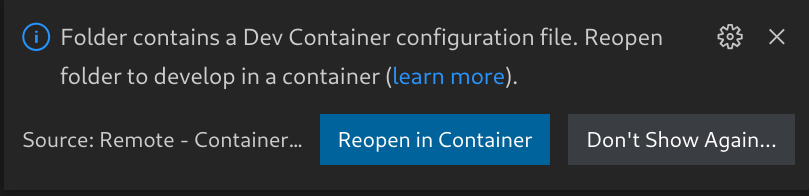
\includegraphics[width=0.55\textwidth]{imgs/dev-container}
        \caption[Mensaje emergente en vscode]{Mensaje emergente en vscode.}
        \label{imgs:vscode-devcontainer2}
    \end{figure}

    \item Fin de la instalación.
\end{enumerate}

\subsection{Instalación basada en docker.}

\paragraph{}\textbf{Nota:} Este método requiere permisos de \emph{sudo} o super usuario
usuario en caso de que docker no esté previamente instalado.

\begin{enumerate}
    \item Instalar \textbf{\gls{git}} (\emph{sólo si es necesario}).
    \begin{lstlisting}[style=consola, numbers=left]
        $ sudo apt install -y git
    \end{lstlisting}

    \item Clonar el repositorio desde github
    \begin{lstlisting}[style=consola, numbers=left]
        $ git clone https://github.com/Gmatarrubia/dev_env_rpi_flutter_yocto.git
        $ cd dev_env_rpi_flutter_yocto
    \end{lstlisting}

    \item (Opcional) En caso de necesitar instalar Visual Studio Code para el desarrollo,
    se puede utilizar la siguente opctión.
    \begin{lstlisting}[style=consola, numbers=left]
        $ source checkFunctions.sh
        $ check_vscode
    \end{lstlisting}

    \item Ejecutar el script inicialización de container. Este script construye la
    imagen en caso de que no haya sido creada previamente.
    \begin{lstlisting}[style=consola, numbers=left]
        $ ./init-docker-env.sh
    \end{lstlisting}
    \textbf{Nota:} Después de este paso podría ser necesario reiniciar, la salida del
    script nos indicará si ésto fuera necesario. Si reiniciamos, sería necesario volver
    a repetir este último paso para que la instalación continue.

    \item Fin de la instalación.
\end{enumerate}

\begin{figure}[H]
    \centering
    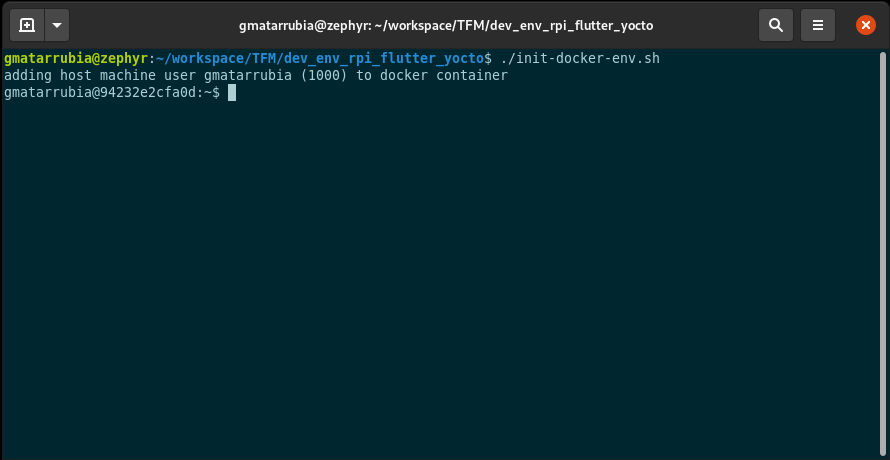
\includegraphics[width=0.95\textwidth]{imgs/yocto-docker-ready}
    \caption[yocto docker ready]{Entorno de desarrollo Yocto listo.}
    \label{imgs:yocto-docker-ready}
\end{figure}

\subsection{Instalación nativa.}

\paragraph{}\textbf{Nota:} Este método requiere permisos de \emph{sudo} o super usuario.

\begin{enumerate}
    \item Instalar la herramienta \textbf{\gls{git}} de control de versiones.
    \begin{lstlisting}[style=consola, numbers=left]
        $ sudo apt install -y git
    \end{lstlisting}

    \item Clonar el repositorio desde github
    \begin{lstlisting}[style=consola, numbers=left]
        $ git clone https://github.com/Gmatarrubia/dev_env_rpi_flutter_yocto.git
    \end{lstlisting}

    \item Ejecutar el script de instalación de paquetes.
    \begin{lstlisting}[style=consola, numbers=left]
        $ cd dev_env_rpi_flutter_yocto
        $ sudo ./installDevDeps.sh
    \end{lstlisting}

    \item (Opcional) En caso de necesitar instalar Visual Studio Code para el desarrollo,
    se puede utilizar la siguente opctión.
    \begin{lstlisting}[style=consola, numbers=left]
        $ source checkFunctions.sh
        $ check_vscode
    \end{lstlisting}

    \item Fin de la instalación.
\end{enumerate}

\subsection{Instalación en sistemas operativos Windows.}

\paragraph{}\textbf{Nota:} Este método es una prueba de concepto y el rendimiento puede
verse visiblemente afectado. Como opción alternativa se aconseja crear una máquina
virtual Ubunut 20.04 y seguir los consejos de la instalación en Linux de manera nativa.

\paragraph{}\textbf{Nota 2:} Se requieren permisos de administrador.

\paragraph{}Los pasos para obtener nuestro entorno de desarrollo listo para trabajar son:

\begin{enumerate}
    \item Instalar y configurar \gls{WSL2}. Para ello, abrir una consola, ya sea cmd
    o powershell, con permisos de administrador e introducir el siguiente comando:
    \begin{lstlisting}[style=cmd, numbers=left]
        wsl.exe --install
    \end{lstlisting}

    \item Reiniciar el sistema.

    \item Arrancar \gls{WSL2} desde el Menú de Inicio. Y realizar la configuración
    inicial que se nos indique, normalmente esto consiste en crear un usuario y
    contraseña.

    \item Una vez en la terminal de \gls{WSL2}, comprobamos que todo haya ido bien realizando
    la actulización de los paquetes de sistema con:
    \begin{lstlisting}[style=consola, numbers=left]
        $ sudo apt update
        $ sudo apt upgrade
    \end{lstlisting}

    \item Siguiendo en la terminal de \gls{WSL2}, instalamos la herramienta git y clonamos
    el repositorio.
    \begin{lstlisting}[style=consola, numbers=left]
        $ sudo apt install -y git
        $ git clone https://github.com/Gmatarrubia/dev_env_rpi_flutter_yocto.git
    \end{lstlisting}

    \item Instalar Visual Studio Code siguiendo la instalación recomendada en su página
    oficial: \href{https://code.visualstudio.com/download}{https://code.visualstudio.com/download}

    \item Abrir Visual Studio Code e instalar las extensiones necesarias. Para ello
    una vez en VSCode, utilizar el atajo de teclado \emph{Ctrl+p} e introducir el siguiente
    comando. Debemos aceptar cualquier sugerencia que nos pregunte:
    \begin{lstlisting}[style=cmd]
        ext install ms-vscode-remote.vscode-remote-extensionpack
    \end{lstlisting}

    \item Abrir un entorno \gls{WSL2} en Visual Studio Code y abrir la carpeta del repositorio
    previamente descargado.
    blabla - insertar captura pantalla.

    \item Ejecutar el script de instalación de paquetes.
    \begin{lstlisting}[style=consola, numbers=left]
        $ cd dev_env_rpi_flutter_yocto
        $ sudo ./installDevDeps.sh
    \end{lstlisting}

    \item Fin de la instalación.
\end{enumerate}

\subsection{Instalación en sistemas operativos MacOS.}

\paragraph{}Blabla

%las referencias a artículos se ponen con \cite,
%las referencias a glosario \gls,
%y las referencias a ecuaciones \eqref
%las referencias a imgenes, tablas o figuras o secciones
% se ponen con \ref (sólo número) o con \hyperref[sec:X]{Blabla}

\chapter{Guía de Uso.}\label{sec:GuiaDeUso}

\paragraph{}En este capítulo se van a explicar las principales funciones del entorno de
desarrollo, así como las principales opciones de cada herramienta provista para los
desarrolladores.

\section{Consideraciones previas.}

\paragraph{}Todos los pasos de todas las guías de este capítulo podrán ser seguidas si
previamente se han seguido las indicaciones del cápitulo \ref{sec:ManualDeInstalacion}.

\paragraph{}Al igual que en el capítulo anterior \ref{sec:ManualDeInstalacion}, la guía
de uso estará dividida en: entorno de desarrollo Flutter y entorno de desarrollo Yocto.
Esta separación lógica, tiene sentido ya que ambas partes pueden funcionar tanto por
separado como juntas. Y ambas partes pueden ser utilizadas para propósitos distintos
que el de funcionar juntas.

\section{Entorno de desarrollo Flutter.}

\paragraph{}Una vez instalado, el uso del entorno Flutter no deja de ser indéntico a
cómo se usa habitualmente Visual Studio Code para el desarrollo de Flutter. Por ello,
si no se está acostumbrado al desarrollo de Flutter en Visual Studio Code, existen
multitud de guías en internet que lo explican, como la se puede encontrar en el
siguiente enlace:

\paragraph{}\href{https://esflutter.dev/docs/development/tools/vs-code}
{Guía oficial de desarrollo de Flutter en Vscode}

\subsection{Características Principales.}

\begin{itemize}
    \item Compatibilidad con la mayoría de sistemas operativos.
    \item Facilidad de instalación.
    \item Fácil de gestionar remotamente.
    \item \gls{IaaC}.
\end{itemize}

\paragraph{}Las principales particularidades de este entorno de desarrollo son las
maneras de inicializar las herramientas para empezar a trabajar. Dicha manera, dependerá
del método de instalación elegido.

\paragraph{}Para empezar a trabajar con el método \emph{desarrollo en container de docker},
cada vez que se abra Vscode habrá que reabrir el proyecto pulsando en el botón del mensaje
emergente que nos aparece al abrir la carpeta de trabajo.

\begin{figure}[H]
    \centering
    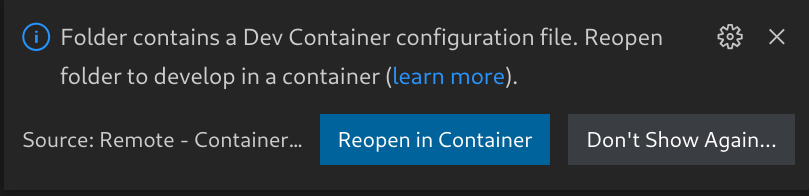
\includegraphics[width=0.75\textwidth]{imgs/dev-container}
    \caption[Mensaje emergente en Vscode]{Mensaje emergente en Vscode.}
    \label{imgs:vscode-devcontainer-2}
\end{figure}

\paragraph{}En caso de que se haya optado por trabajar desde el entorno \emph{Dockerizado}
sólo habrá posibilidad de realizar las siguientes acciones: compilar, ejecutar la aplicación,
lanzar los test y depurar con las opciones del servidor de depuración a través del navegador.
Todas estas acciones salvo la última se realizan por línea de comandos. La depuración,
será limitada y para acceder a ella, debemos abrir en el navegador la IP indicada.

\begin{figure}[H]
    \centering
    \fbox{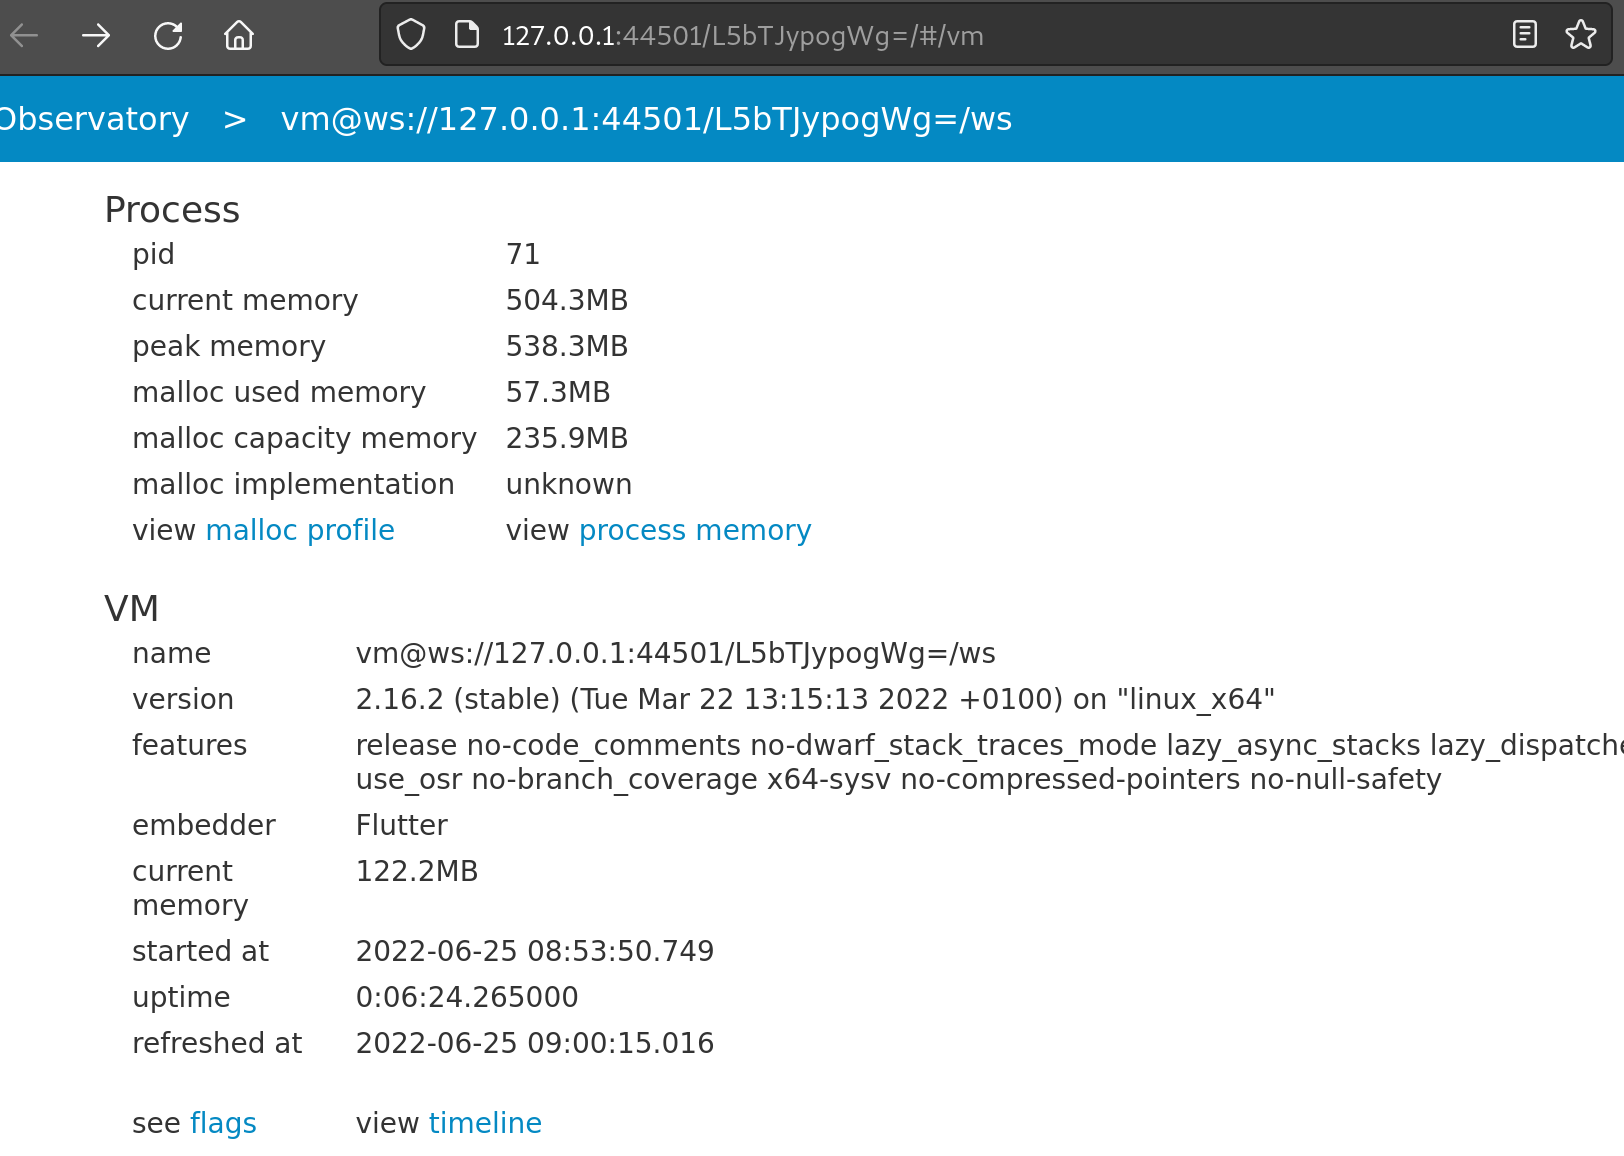
\includegraphics[width=0.75\textwidth]{imgs/devtools}}
    \caption[Navegador con devtools]{Navegador con devtools.}
    \label{imgs:devtools}
\end{figure}

\paragraph{}Si estamos utilizando el entorno en Windows con \gls{WSL2}, entonces una
vez arrancado el entorno \gls{WSL2} debemos arrancar un cliente de escritorio remoto
para visualizar la aplicación.

\begin{figure}[H]
    \centering
    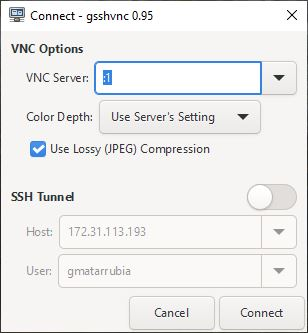
\includegraphics[width=0.40\textwidth]{imgs/gsshvnc-open}
    \caption[Abriendo el cliente gsshvnc]{Abriendo el cliente gsshvnc.}
    \label{imgs:open-gsshvnc}
\end{figure}

\begin{figure}[H]
    \centering
    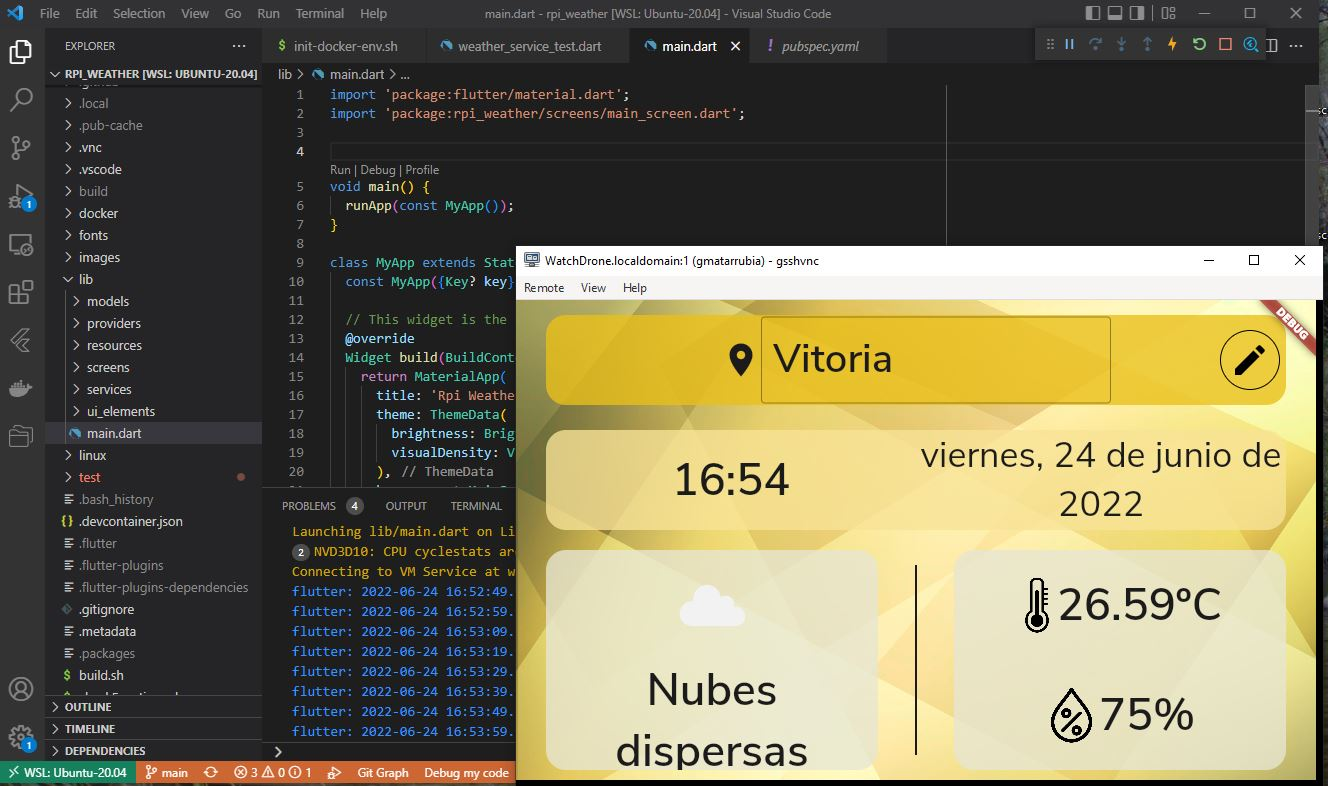
\includegraphics[width=0.90\textwidth]{imgs/wsl2-running}
    \caption[WSL2 + gsshvnc.c]{WSL2 + gsshvnc.}
    \label{imgs:running-gsshvnc}
\end{figure}

\paragraph{}A continuación se muestran las acciones provistas por el entorno de desarrollo.

\subsection{Build.}

\paragraph{}Para compilar la aplicación se puede utilizar el siguiente comando por
terminal:

\begin{lstlisting}[style=consola, numbers=left]
    # Usage of ./build.sh [--debug] | [--test]
    $ ./build.sh
\end{lstlisting}

\paragraph{}Como podemos observar, el comando acepta los argumentos: \emph{debug} y
\emph{test}. Por defecto, la aplicación se compila en \gls{release}, salvo que pasemos
el argumento de \emph{debug}. El argumento \emph{test}, se utilizará para compilar y
ejecutar los test. Este argumento invalida al anterior.

\subsection{Ejecutar la app.}

\paragraph{}Este comando nos permite ejecutar la aplicación desde una terminal.

\begin{lstlisting}[style=consola, numbers=left]
    # Usage of ./runApp.sh [--debug] | [--release]
    $ ./runApp.sh
\end{lstlisting}

\paragraph{}Los argumentos que admite este comando son: \gls{debug} y \gls{release}.
Ambos se corresponden con los modos de ejecución de la aplicación. En caso de querer
ejecutarla y que ésta no haya sido compilada previamente se compilará con el modo
correspondiente antes de ser ejecutada. Por defecto, la app se ejecuta en modo \gls{release}.

\subsection{Limpiar repo.}

\paragraph{}Con este comando limpiaremos todos los archivos que habían sido generados
automáticamente.

\begin{lstlisting}[style=consola, numbers=left]
    $ ./cleanAll.sh
\end{lstlisting}

%%%%%%%%%%%%%%%%%%%%%%%%%%%%%%%%%%%%%%%%%%%%%%%%%%%%%%%%%%%%%%%%%%%%%%%%%%%%%%%%%%%%%%

\section{Entorno de desarrollo Yocto.}

\paragraph{}Este es el entorno de desarrollo de la distribución FlutterPI. Una distribución
con el kernel de linux para Raspberry Pi basada en Poky (Yocto) la cuál está pensada
para correr aplicaciones de Flutter. Esto es muy útil para múltiples aplicaciones como
por ejemplo: Máquinas de vending, paneles de información, y muchísimos otros tipos de
HMIs. Este entorno de desarrollo permite tomarlo de plantilla y desarrollar rápidamente
un sistema HMI, fiable, replicable y altamente personalizable.

\subsection{Características principales.}

\paragraph{}Este entorno ha sido diseñado teniendo en cuanta los siguiente aspectos:

\begin{itemize}
    \item Compatibilidad con la mayoría de sistemas operativos.
    \item Facilidad de uso.
    \item Entendible y bien documentado.
    \item Fácil de gestionar remotamente.
    \item Flexibilidad y multipropósito.
    \item \gls{IaaC}.
\end{itemize}

\paragraph{Nota:} Este entorno corre nativamente en sistemas con distribuciones Ubuntu 20.04.
Para el resto de sistemas utilizar cualquiera de los métodos alternativos:

\begin{itemize}
    \item Entorno dockerizado.
    \item Máquina virtual con Ubuntu 20.04.
    \item Entorno en WSL2 (sólo para sistemas Windows 10/11.)
\end{itemize}

\paragraph{}Acudir al capítulo \hyperref[sec:ManualDeInstalacion]{Manual de instalación}
\ref{sec:ManualDeInstalacion} antes de intentar los procedimientos descritos en este
capítulo.

\subsection{Build.}

\paragraph{}Para lanzar la generación de la imagen completa con las configuraciones por
defecto utilizar el siguiente comando. El resultado será una imagen arrancable en una
Raspberry Pi el cuál arrancará una aplicación Flutter al comienzo.

\begin{lstlisting}[style=consola, numbers=left]
    $ ./build.sh
\end{lstlisting}

\paragraph{}Antes de empezar la generación, el entorno te preguntará la configuración
Wi-Fi para conectarse a un punto de acceso (ssid + pass). Ésto se puede saltar si
previamente se han configurado las variables de entorno: \emph{WIFISSID} y \emph{WIFIPASS}.

\paragraph{}Para más información sobre los aspectos del script de build pueden ser
consultados con el comando:

\begin{lstlisting}[style=consola, numbers=left]
    $ ./build.sh --help
    This script help you with the initial configuration and with the build process.
    you can use this script with these options:

    -v | --verbose) Prints more detailled output.

    -bc | --bitbake-cmd) Performs your custom bitbake/devtool command.

    --shell) Opens a bitbake shell without do anything else.

    -wi | --wifi-interactive) For setting Wi-Fi settings.

    -d | --debug) Enables debug features on the local.conf

    -h | --help) Prints this useful help :)
\end{lstlisting}

\subsection{Comando de build personalizados.}

\paragraph{}Mediante los argumentos -bc <"custom command"> o --bc <"custom command">,
se puede pasar un comando personalizado al entorno de Yocto. Ésto es especialmente útil
para pasar comandos como: bitbake, bitbake-getvar o devtool por citar unos pocos. Para
hacerse una mejor idea de los usos que puede tener, se presentan unos ejemplos:

\begin{lstlisting}[style=consola, numbers=left]
    # Comando para ver las versiones de todas las recipes de flutter
    $ ./build.sh --bitbake-cmd "bitbake -s | grep flutter"

    # Comando para hacer "clean" de la compilacion de una recipe especifica
    $ ./build.sh -bc "bitbake -D wifi -c clean"

    # Comando para ver las capas analizadas y su preferencia
    $ ./build.sh --bitbake-cmd "bitbake-layers show-layers"
\end{lstlisting}

\subsection{Lanzar el modo Sesión Interactiva.}

\paragraph{}Esta es una manera potente de depurar y desarrollar tus recipes o tus
aplicaciones flutter. Ya que abres una terminal en la que puedes lanzar comandos como
los anteriores de manera interactiva e iterativa. También da acceso a usar el \gls{eSDK}.

\begin{lstlisting}[style=consola, numbers=left]
    $ ./build.sh --shell
\end{lstlisting}

\paragraph{}Algunos ejemplos de comandos que puedes utilizar dentro de la terminal interactiva:

\begin{itemize}
    \item bitbake
    \item bitbake-getvar
    \item bitbake-layers
    \item devtool
\end{itemize}

\subsection{Limpieza.}

\paragraph{}Se proveé del siguiente comando para borrar la mayoría de los archivos generados
automáticamente.

\begin{lstlisting}[style=consola, numbers=left]
    $ ./cleanAll.sh
    # Para una limpieza total usar el siguiente comando.
    # Usar con precaucion ya que se pederan todos los cambios no guardados en git.
    $ git clean -fdx
\end{lstlisting}


%las referencias a artículos se ponen con \cite,
%las referencias a glosario \gls,
%y las referencias a ecuaciones \eqref
%las referencias a imgenes, tablas o figuras o secciones
% se ponen con \ref (sólo número) o con \hyperref[sec:X]{text}

\chapter{Aplicación Meteorológica.}\label{sec:AplicacionMeteorologica}

\paragraph{}En este capítulo se va a exponer toda la documentación técnica del diseño
y la arquitectura del software de la aplicación que usaremos de ejemplo para utilizar
el entorno de desarrollo.

\begin{figure}[H]
	\centering
	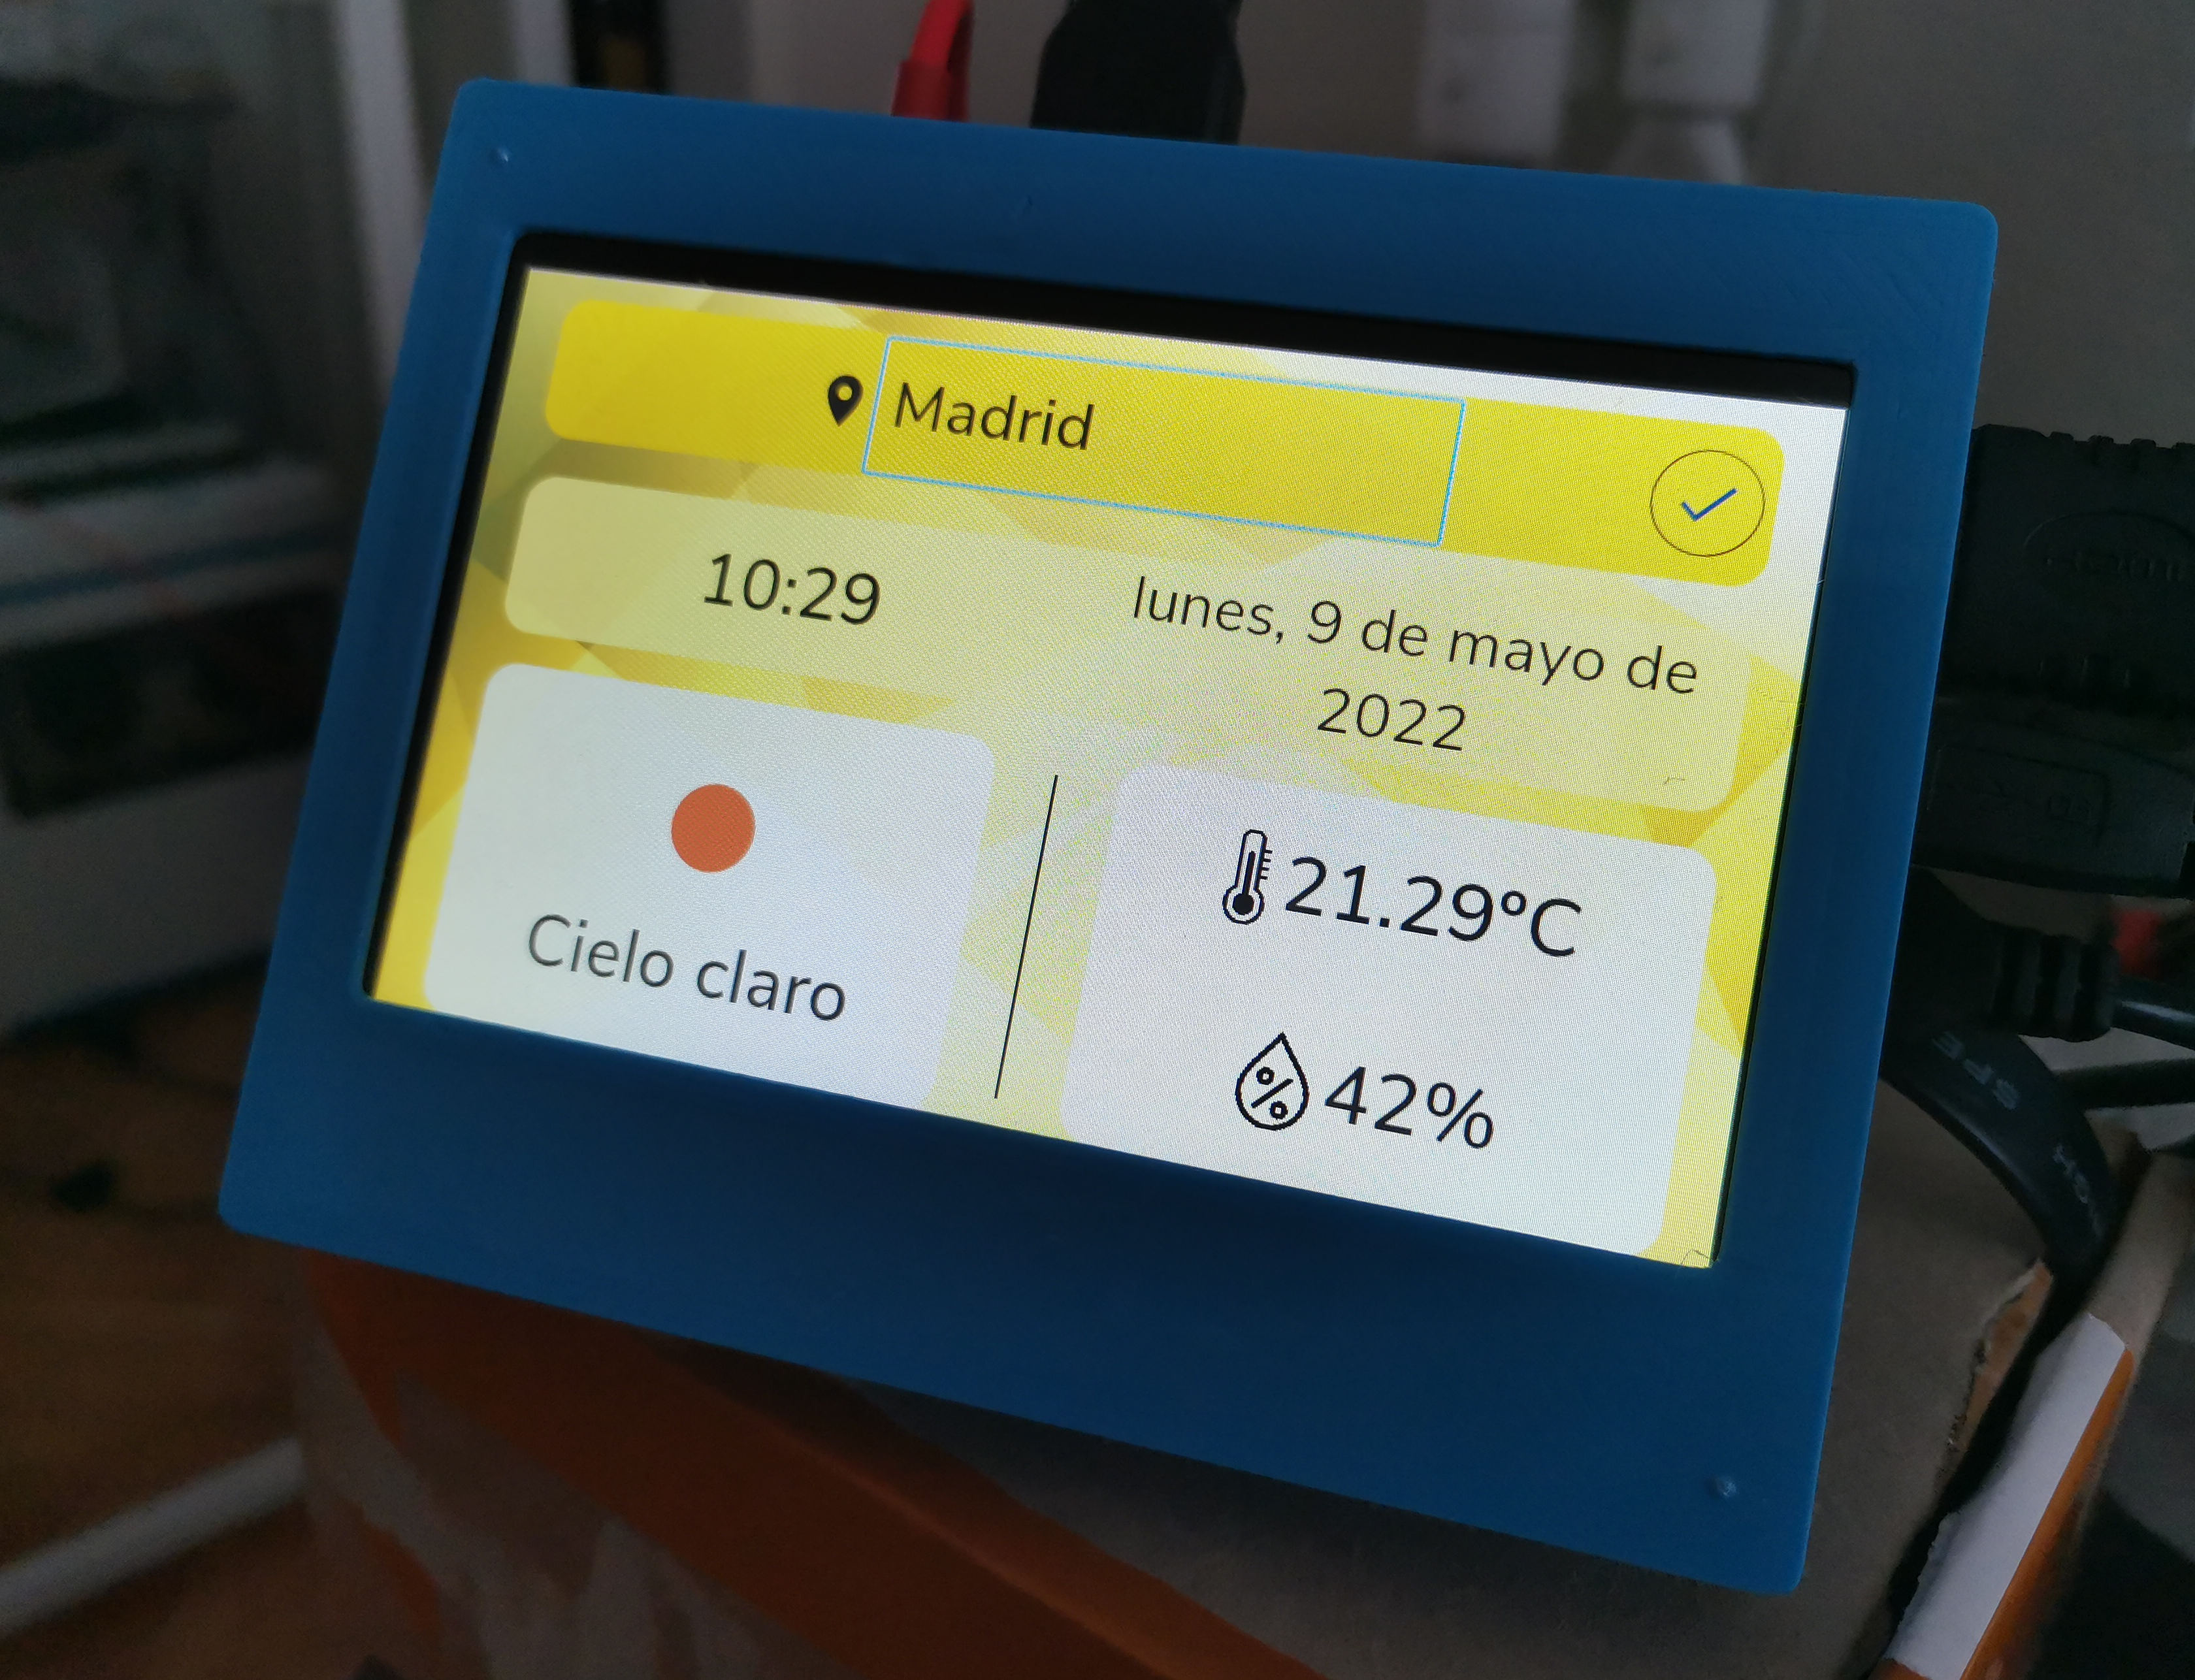
\includegraphics[width=0.9\linewidth]{imgs/app1}
	\caption[Portada de la app]{Fotografía de la aplicación en ejecución.}
	\label{img:rpi-weather-portada}
\end{figure}

\section{Requisitos}

\paragraph{}En esta sección se describirán los requisitos utilizados para el diseño
de la aplicación.

\subsection{Requisitos de usuario:}
\begin{itemize}
    \item Como usuario, quiero disponer de la fecha y hora en todo momento.
    \item Cómo usuario, quiero disponer de la información meteorológica de cualquier
    ciudad del mundo.
    \item Como usuario, quiero poder elegir la ciudad de la que quiero conocer la
    información meteorlógica.
\end{itemize}

\subsection{Requisitos funcionales:}
\begin{itemize}
    \item Se debe mostrar la información con la fecha, la hora y la información meteorlógica
    en todo momento.
    \item Como información meteorológica se debe mostrar: temeperatura, humedad, icono
    y breve descripción del estado actual.
\end{itemize}

\subsection{Requisitos no funcionales:}

\subsubsection{Requisitos de precisión:}
\begin{itemize}
    \item La hora mostrará horas y minutos en formato 24: HH:MM.
    \item La fecha debe mostrar: día de la semana, día del mes, mes y año.
    \item La temperatura se mostrará en grados centígrados con dos decimales de precisión.
    \item La humedad se representará con números enteros en tanto por ciento.
\end{itemize}

\subsubsection{Requisitos de rendimiento:}
\begin{itemize}
    \item La información debe actualizarse con una frecuencia mínima de 10 segundos y
    siendo deseable una frecuencia aproximada de 1 segundo.
\end{itemize}

\subsubsection{Requisitos de disponibilidad:}
\begin{itemize}
    \item La información debe mantenerse visible en todo momento mientras el sistema
    permanezca encendido.
    \item El sistema debe iniciarse tan pronto como se conecte a una fuente de energía.
\end{itemize}

\subsubsection{Requisitos de manejabilidad:}
\begin{itemize}
    \item La interfaz debe manejarse de manera táctil.
\end{itemize}

\subsubsection{Requisitos de recuperabilidad:}
\begin{itemize}
    \item Al encenderse, el sistema debe mostrar la información meteorológica de la
    última ciudad fijada.
\end{itemize}

\subsection{Requisitos de Interfaces externas:}

\subsubsection{Interfaces de usuario:}
\begin{itemize}
    \item Toda la información debe ser mostrada en un display de 5" táctil.
    \item El display permitirá el cambio de ubicación mediante uso del táctil de la pantalla.
\end{itemize}

\subsubsection{Interfaces de comunicaciones:}
\begin{itemize}
    \item El disposivo requerirá acceso a internet para obtener las métricas.
    \item El acceso a internet puede ser provisto por una interfaz ethernet (cableada)
    o Wi-Fi (sin cables).
\end{itemize}

\section{Casos de Uso}

\paragraph{}En esta sección se describen los casos de uso extraídos de los requisitos
mediante un diagrama formal SysML.

\begin{figure}[H]
	\centering
	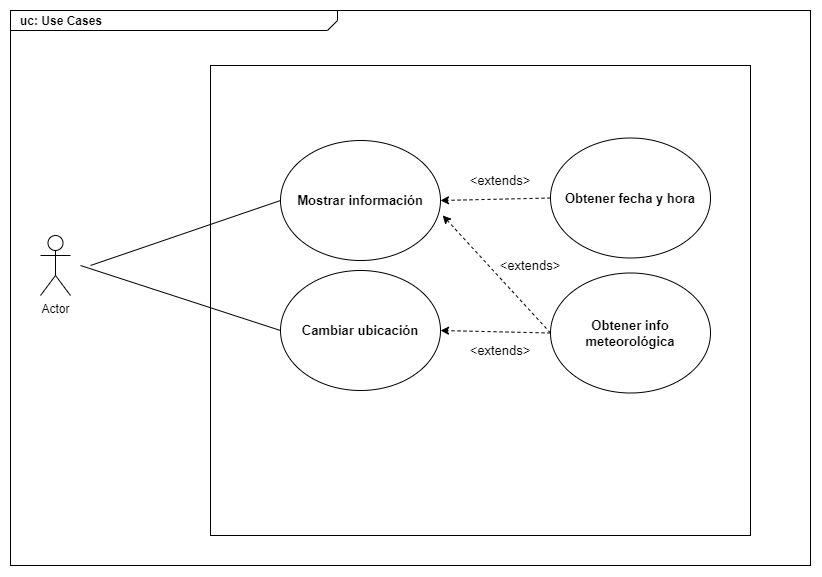
\includegraphics[width=0.9\linewidth]{figs/rpi_weather-uc}
	\caption[Diagrama SysML de casos de uso]{Diagrama SysML de casos de uso.}
	\label{fig:use_cases}
\end{figure}

\section{Diseño de interfaz de usuario}

\paragraph{}La interfaz de usuario en este caso se compone únicamente de una pantalla
táctil. Los diseños mostrados en esta sección, pertenecen al diseño original hecho en
Figma, un servicio online de diseño especializado en interfaces de usuario. Por eso mismo,
pueden existir pequeñas variaciones con el diseño final mostrado en la implementación final.

\paragraph{}\textbf{Pantalla principal:}

\begin{figure}[H]
	\centering
	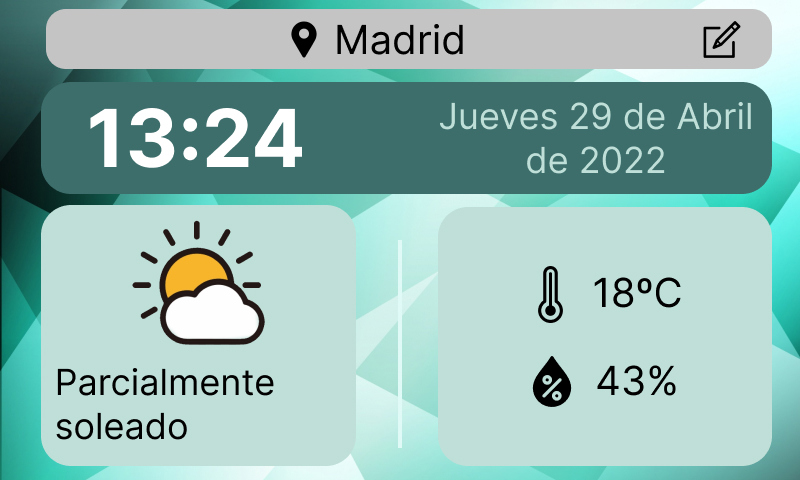
\includegraphics[width=0.75\linewidth]{imgs/figma-main}
	\caption[Diseño de la pantalla principal]{Diseño de la pantalla principal}
	\label{fig:design_main_screen}
\end{figure}

\paragraph{}\textbf{Edición de la localización:}

\begin{figure}[H]
	\centering
	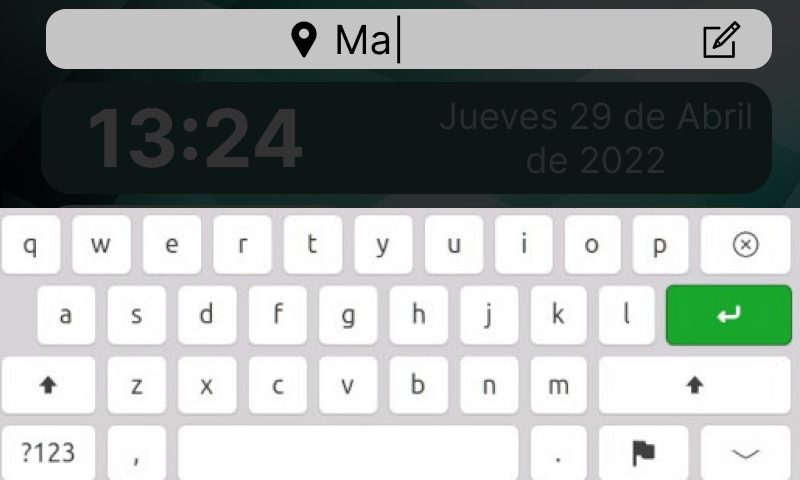
\includegraphics[width=0.75\linewidth]{imgs/figma-location}
	\caption[Diseño del cambio de localización]{Diseño del cambio de localización}
	\label{fig:design_location}
\end{figure}

\section{Arquitectura}

\paragraph{}La arquitectura de esta aplicación utiliza un patrón MVC modificado con el
patrón \emph{Change Notifier}. Esta arquitectura se caracteriza por manejar de forma
eficiente el estado de la aplicación. Las \emph{views} se suscriben a proveedores de
estado de los modelos que necesitan. Y cuando cambia el estado del modelo suscrito,
estas vistas se regeneran. Las vistas, a su vez pueden servir para cambiar el estado
de los modelos, previo tratamiento de los \emph{inputs} por la lógica de negocio provista
por los controladores.

\begin{figure}[H]
	\centering
	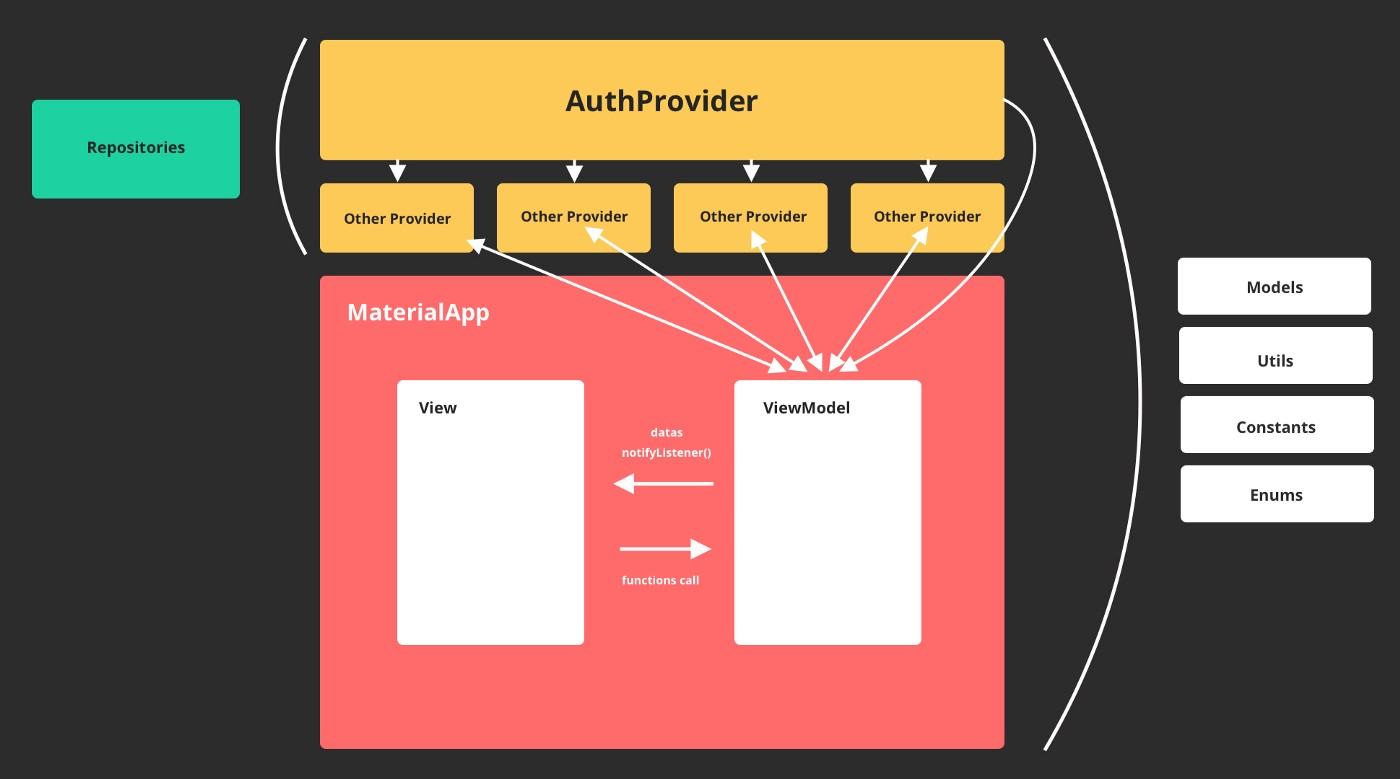
\includegraphics[width=0.85\linewidth]{figs/change-notifier}
	\caption[Arquitectura ChangeNotifier]{Diagrama de arquitectura Change Notifier.}
	\label{fig:ChangeNotifier}
\end{figure}

\paragraph{}En la figura \ref{fig:provider} mostrada a continuación, encontramos un
diagrama de clases genérico que explica como es la implementación del patrón de diseño
provider.

\begin{figure}[H]
	\centering
	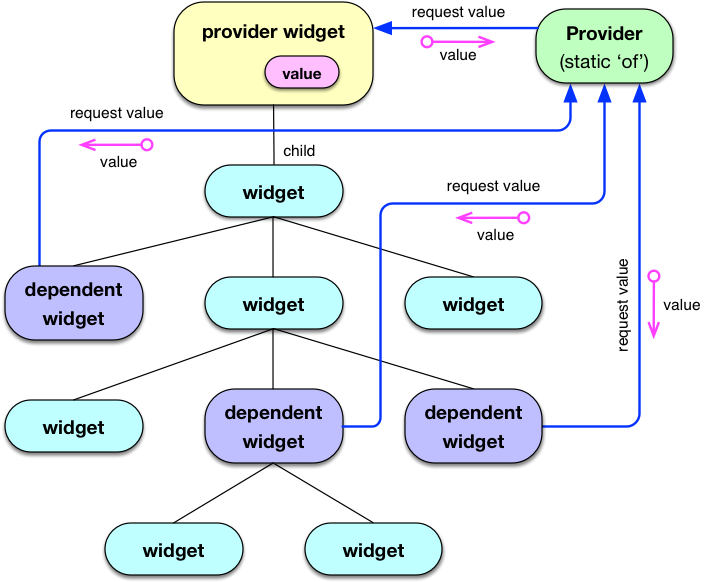
\includegraphics[width=0.75\linewidth]{figs/provider-pattern}
	\caption[Patron Provider]{Diagrama de clases con patrón provider.}
	\label{fig:provider}
\end{figure}

\subsection{Diagrama de clases}

\paragraph{}En la figura \ref{fig:classDiagram} se muestra el diagrama de clases de la
aplicación de meteorología implementada. El diagrama está algo simplificado para facilitar
la lectura y comprensión, sin embargo, representa fielmente la implementación.

\begin{figure}[H]
	\centering
	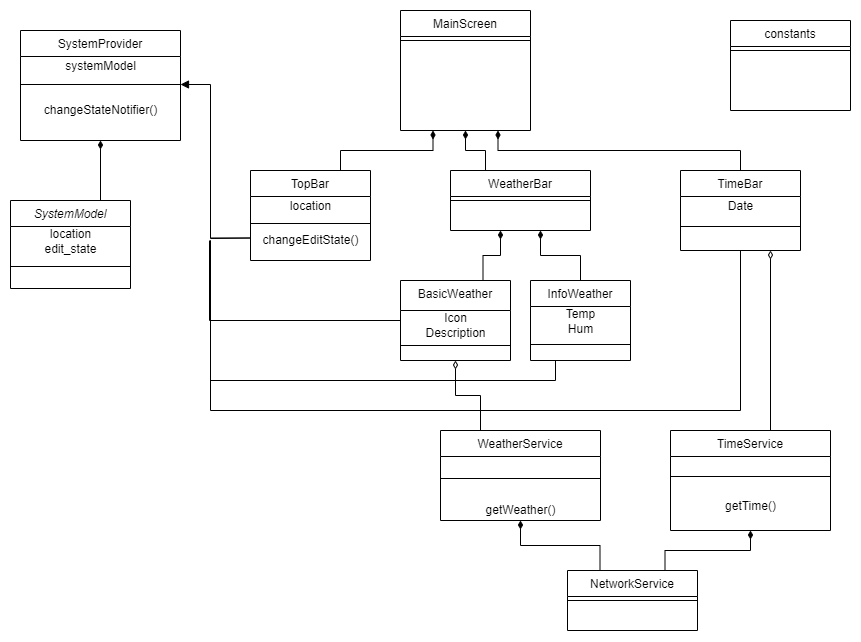
\includegraphics[width=0.95\linewidth]{figs/rpi_weather-class_diagram}
	\caption[Patron Provider]{Diagrama de clases con patrón provider.}
	\label{fig:classDiagram}
\end{figure}

\paragraph{}Como ya se ha dicho con anterioridad, esta aplicación se diseño para servir
de ejemplo o demostrador del entorno de desarrollo. El uso de aplicaciones flutter en
entornos embebidos y basado en Yocto no está muy extendido. No obstante, esto es sobre
todo debido a la falta de documentación, ya que queda demostrado cuan práctico y
conveniente puede llegar a ser.

\paragraph{}Al ser un demostrador,se ha querido documentar como si de una plantilla o
\emph{template} se tratase. También se han desarrollado unos cuantos test, para la
demostración del entorno de testing. Vale la pena recordar, que la aplicación en sí
misma es independiente del entorno de desarrollo y del proyecto Yocto que la usa.

\paragraph{}Todo el código de la aplicación y la presentación básica en inglés puede
encontrarse en el siguiente repositorio de código público:

\paragraph{}\href{https://github.com/Gmatarrubia/rpi_weather}{github.com/Gmatarrubia/rpi weather}


%las referencias a artculos se ponen con \cite,
%las referencias a imgenes \ref,
%las referencias a glosario \gls,
%y las referencias a ecuaciones \eqref

\chapter{Desarrollo de la Aplicación.}\label{sec:Desarrollo}

\paragraph{}En este capítulo vamos a conectar el uso teórico del entorno de desarrollo
mostrado en el capítulo \ref{sec:GuiaDeUso}, con el diseño software y la arquitectura de
la aplicación meteorológica del capítulo \ref{sec:AplicacionMeteorologica}. Lo haremos
explicando cómo ha sido el desarrollo de la aplicación en con el entorno de desarrollo.

\section{Ejecutando la aplicación de inicio}

\paragraph{}Blabla

\section{Generación de imagen de disco y prueba en hardware.}

\paragraph{}Blabla

\section{Primeros cambios y depuración "Hot debbuging".}

\paragraph{}Blabla

\section{Ejecutando los test unitarios.}

\paragraph{}Blabla

%las referencias a artculos se ponen con \cite,
%las referencias a imgenes \ref,
%las referencias a glosario \gls,
%y las referencias a ecuaciones \eqref

\chapter{Integración en sistemas CI/CD}\label{sec:cicd}

\paragraph{}Cuando hablamos de sistemas \gls{CI/CD} nos solemos referir a todos aquellos
servidores, servicios y máquinas; ya sean \gls{on premises} o en cloud, que posibilitan
el desarrollo centralizado, el control de versiones, el aseguramiento de la calidad
y la entrega continua.

\begin{figure}[H]
    \centering
    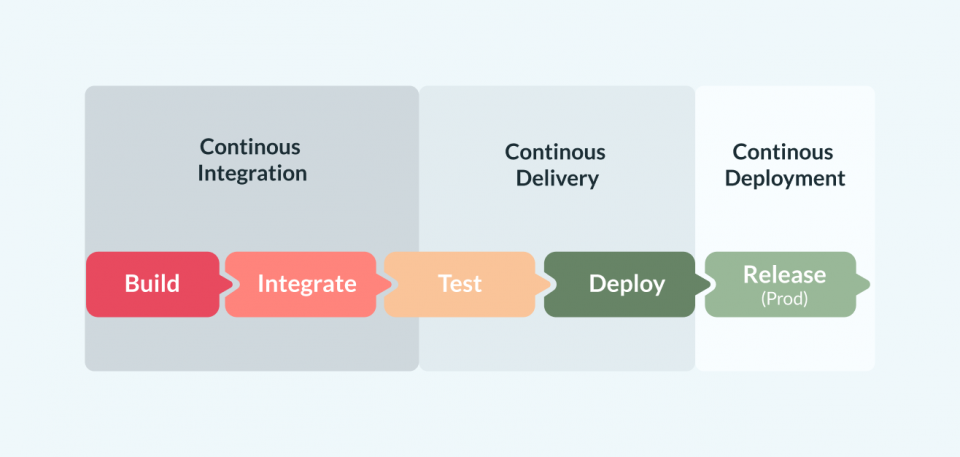
\includegraphics[width=0.75\textwidth]{imgs/cicd}
    \caption{Esquemas de estrategia CI/CD.}
    \label{imgs:cicd}
\end{figure}


\paragraph{}\textbf{Nota: }\emph{Cómo entrar en detalle en estos apartados sería extender
demasiado el alcance que se prentende en este trabajo, este capítulo se va a limitar a
describir la relación del entorno de desarrollo con los sistemas \gls{CI/CD}. Cualquier
arquitectura de la infraestructura es pura expeculación y no será probada a nivel práctico.}

\section{Control de versiones}

\paragraph{}El control de versiones en este entorno de desarrollo se realiza mediante
\gls{git}. \Gls{git} es una herramienta de control de versiones gratuita, multiplataforma que
es muy popular, tanto que incluso podría empezar a considerarse un estandar. Populares
servicios de repositorios online, como \href{github.com}{github} o \href{gitlab.com}{gitlab}
funcionan con este sistema. Para este proyecto, se ha elegido \href{github.com}{github}
por su popularidad. Ya que al ser código abierto, esto facilita que más desarrolladores
encuentren el proyecto e incluso quieran colaborar para hacer sus aportaciones. Además,
github permite aplicar la política de branching GitHub-Flow, la cual explicaremos más
adelante en detalle.

\paragraph{}En mi experiencia laboral, he utilizado \gls{git} en repositorios compartidos
por más de mil desarrolladores y \gls{git} facilita la gestión del control de versión.
Obviamente, en casos tan ``extremos'' como el mencionado, existen carencias que no
resuelve la propia herramienta, y que han de ser solventados mediante la implantación
de protocolos internos y patrones de branching.

\paragraph{}Algunos de los patrones más utilizados son: patrón release-ready mainline,
hot-fix branch, feature branch, release branch o production branch. Estos patrones deben
ser implementados en función de la naturaleza del proyecto, de la cantidad de cambios que
sufre el código, la metodología de desarrollo de la empresa, de la relación con el
cliente, etc.

\subsection{Ciclo de vida del desarrollo software}

\paragraph{}Como se puede apreciar en la imagen \ref{imgs:recipe-rpi-weather-1} cada
vez que se haga un \gls{fetch} de Rpi Weather, se va a descargar lo último que haya en la
rama principal. Esto tiene unas consecuencias inmediatas. La rama principal debe contener
en todo momento código funcional dispuesto a ser entregado y que pase todas las pruebas
necesarias. En un entorno real, lo más conveniente sería fijar la referencia de una recipe,
o bien a un \emph{tag} o \emph{commit} concretos o bien a una rama de release. Pero para
nuestro ejemplo, vamos a considerar la rama \emph{main} como una rama de release.

\begin{figure}[H]
    \centering
    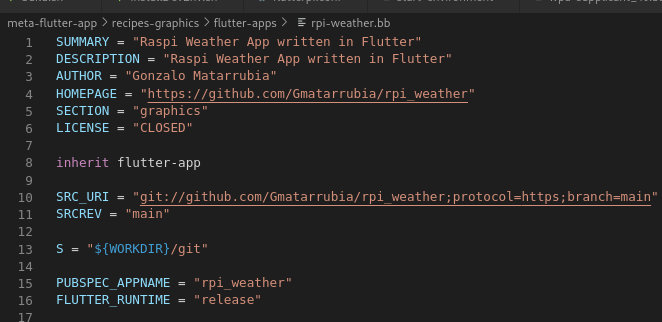
\includegraphics[width=0.90\textwidth]{imgs/rpi-weather-recipe}
    \caption[Detale recipe de Rpi Weahter]{Detalle de la recipe de Rpi Weather.}
    \label{imgs:recipe-rpi-weather-1}
\end{figure}

\paragraph{}Yocto admite tener tanto fuentes locales, como fuentes en servidores. Por
eso mismo, para el desarrollo de la aplicación flutter se propone el uso de los
siguiente patrones de branching, explicando sus fundamentos.

\paragraph{Política de branching GitHub-Flow:} Está política de branching agrupa unos
cuantos patrones que adapta a su plataforma online. GitHub-Flow está orientado a proyectos
con una sola versión en producción y una alta frecuencia de integraciones en la rama
principal, la cual será una \emph{Release-Ready Mainline}\ref{sec:release-ready}. En
principio las release branch no son necesarias, ni tampoco las Hotfix branch, éstas
últimas existiran pero no será diferentes de una feature branch normal. Nadie trabajará
en la rama principal, cada característica/función/mejora debe hacerse en una \emph{feature
branch}. Dicha función o mejora debe estar acotada y una vez terminada, se hará una
\emph{pre-integration review}, es decir que se revisarán los cambios que se quieren
introducir en la rama principal. Una vez revisados y aprobados los cambios, es común
que se realice una serie de comprobaciones automáticas y en caso de éxito, se integren
los cambios en la rama principal. Las comprobaciones automáticas pueden incluir, análisis
dinámico y/o estático de código, test unitarios, test de integración, compilación, etc.
En Github, esta revisión tiene su propia herramienta llamada \emph{Pull Request}.

\begin{figure}[H]
    \centering
    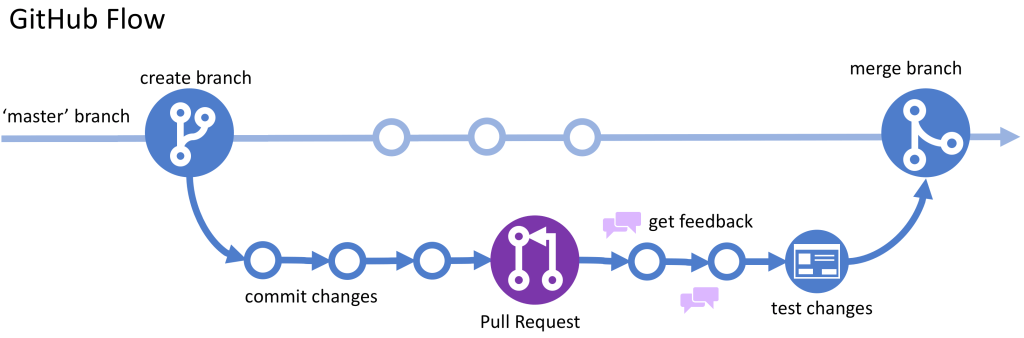
\includegraphics[width=0.85\textwidth]{imgs/github-flow}
    \caption{Esquema de una rama en Github Flow}
    \label{imgs:github-flow}
\end{figure}

\paragraph{Patrón Release-ready Mainline:}\label{sec:release-ready}

\paragraph{}Como su propio nombre indica, este patrón de branching nos indica que cada
\emph{commit} hecho en la línea principal o \emph{mainline} debe poder ser liberado a
producción. No obstante, conviene aclarar que el hecho de que pueda ser ``liberable'',
no significa que tenga que serlo. Dependera de si la empresa practica el \emph{continuous
deployment} o \emph{continous delivery}, en este último caso serán las decisiones de
negocio las que decidirán que versión desplegar a producción de entre todas las versiones.


\paragraph{Patrón Feature branch:} Una feature branch se utilizará para conjuntos de
cambios que tengan una relación lógica. Los objetivos de una feature branch, deben ser
medibles y finitos. De menera que cada característica nueva del programa, cada bug, etc
esté en su propia rama exclusiva.

\subsection{Infraestructura}

\paragraph{}Normalmente, los sistemas de control de versiones están ``supervisados''
por equipos de compilación, analizadores estáticos y dinámicos, despligue de artefactos,
etc. Es decir, que existe una infraestructura que trabaja de forma automatizada con
nuestro código y los cambios que le introducimos. Esta infraestructura puede estar
en local, \gls{on premises} o en cloud. Lo único que cambia en cada caso es la hubicación
física del \emph{hardware}, así como la responsabilidad de mantener el servicio.

\paragraph{}Para asegurar la mantenibilidad de esta infraestructura, así como para aplicar
las mismas técnicas de desarrollado que se hacen con el código se llevan a cabo descripciones
de \glsplural{pipeline} en lo que se conoce como \gls{IaaC}. De esta manera, el desarrollo
del entorno de desarrollo, valga la redundancia, y sus dependencias puede ser desarrollado
y administrado a la vez y de igual manera que el propio código que contiene.

\paragraph{}Las \glsplural{pipeline} pueden estar contenidas en el propio repositorio
junto al código, lo cual traza una estrategia de infraestructura orientada al proyecto,
o puede estar en un repositorio a parte de manera que pueda ser utilizada en común con
otro proyecto.

\paragraph{}Los \glsplural{pipeline} sólo definen las acciones a realizar en la infraestructura
en determinados eventos, pero la propia definición de la infraestructura también puede
estar definida en código. En nuestro proyecto, los repositorios están pensados para
integrarse en una infraestructura \gls{IaaC} mediante Ansible\ref{sec:ansible}. En este
proyecto, por su alcance, se han definido unos \emph{playbooks} o unidades de configuración,
implementación y aprovisionamiento reutilizables, en las que deben ser lanzados de forma
local. De esta forma, no habría mucha diferencia con un script normal, más haya de la
sintaxis y el uso de ciertos módulos pre-integrados. En cambio, aplicado Ansible a toda
la infraestructura podría facilitar la preparación de los equipos dónde se a desarrollar
los diferentes entornos, así como las máquinas donde se van a procesar los entornos.

\paragraph{}Con Ansible, por ejemplo, sería muy fácil crear dispositivos nuevos para
nuevos trabajadores que fueran a utilizar los diferentes entornos, aplicando de manera
automática los \emph{playbooks} necesarios en cada caso. Incluso si se realizara un
cambio de requisito y/o entorno, con Ansible podría administrarse todos los equipos,
por lotes y de forma automática y remota.

\section{QA}

\paragraph{}Los mecanismos de infraestructura recomendados para cada entorno cambian.
Como no hay muchas herramientas externas de yocto que permitan hacer un análisis más
avanzado del que hace el propio yocto al generarse, para ese entorno uno o varios nodos
que tengan un servicio de generación centralizado sería suficiente. Incluso se podría
tener un entorno de pre-producción y comprobar la integración hardware como parte del
proceso de \emph{quality assurance}. Los nodos de generación automática podrían utilizar
Jenkins para esta tarea, o bien un alternativa sería utilizar los recursos de GitHub
Actions. Quizás el factor más importante en este caso sería si esta parte de la
infraestructura se quiere hacer el could o \gls{on-premises}. En ambos casos, se
describiría la una \gls{pipeline} en un archivo específico en el propio repositorio de
código.

\begin{figure}[H]
    \centering
    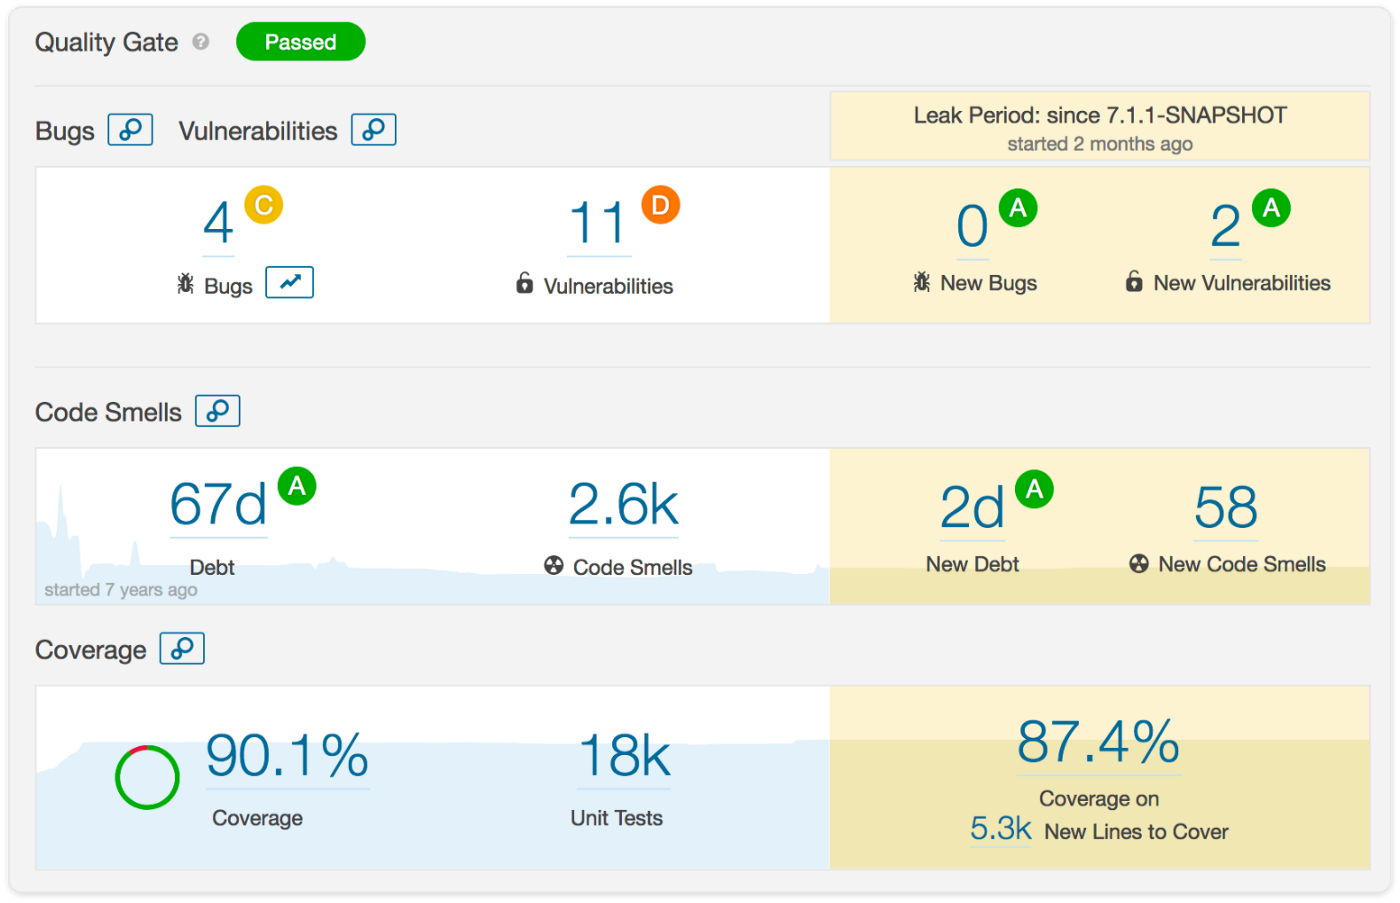
\includegraphics[width=0.85\textwidth]{imgs/sonarqube}
    \caption{Panel principal de Sonarqube}
    \label{imgs:sonarqube}
\end{figure}

\paragraph{}El entorno Flutter admite más variaciones en cuanto a el uso de infraestructura
para gestionar el \emph{quality assurance}. Puede haber nodos de compilación automática,
pero también nodos de análisis de código y ejecución de test. Por ejemplo, se puede
utilizar una instancia de Sonarqube, para obtener resultados acerca de la calidad y del
código, abarcando desde el uso del \gls{coding standard} hasta la deteción de vulnerabilidades.

\paragraph{}El QA siempre tiene una componente subjetiva y que difícilmente se puede
automatizar, así además de medios, para garantizar una buena calidad se necesitan
trabajadores cualificados para dicha tarea.

\section{Entrega continua}

\paragraph{}Hay varias soluciones comerciales que se integran con Yocto para realizar
la entrega continua, tanto para la actualización de la aplicación Flutter dentro del
sistema como para realizar un \emph{full-upgrade} a todo el firmware. En el caso de
querer realizar las actualizaciones \gls{OTA} solo para la aplicación flutter se tienen
más alternativas, ya que podríamos modificar el sistema operativo para instalar cualquier
servicio que aporte esta utilidad. En el caso de querer realizar un \emph{full-upgrade}
es necesario contar con determinadas características del hardware.

\paragraph{}Las estategias más frecuentes para realizar un ``\emph{full-upgrade}'' son:
un disco de arranque de actualización/recuperación o el uso de un hipervisor. Dentro de
los hipervisores, podemos utilizar uno tipo 1 o baremetal, y otro tipo 2, con un sistema
operativo \emph{host} y otro \emph{guest}.

\begin{figure}[H]
    \centering
    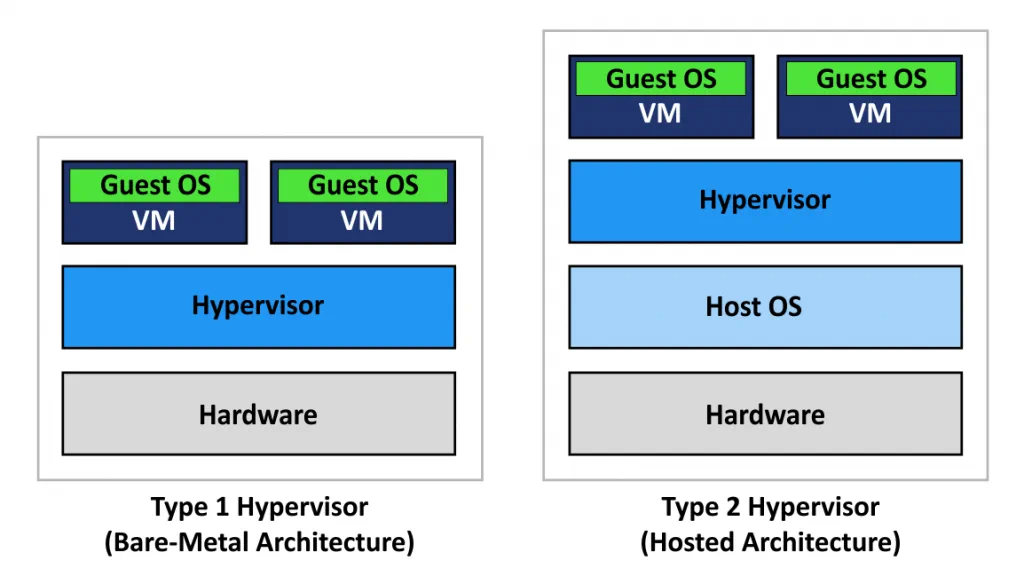
\includegraphics[width=0.75\textwidth]{imgs/hypervisor}
    \caption{Esquemas de los tipos de hipervisor.}
    \label{imgs:hipervisor}
\end{figure}

%las referencias a artculos se ponen con \cite,
%las referencias a imgenes \ref,
%las referencias a glosario \gls,
%y las referencias a ecuaciones \eqref

%\chapter{Cmo escribir en Latex}

\section{Citas}

%las referencias a artculos se ponen con \cite,
%las referencias a imgenes \ref,
%las referencias a glosario \gls,
%y las referencias a ecuaciones \eqref

Esto es un ejemplo de cita de un artculo \cite{Brunete:2013}.


\section{Listas}

%itemize es una lista. Cada trmino lleva delante un \item
Ejemplo de lista de puntos:
\begin{itemize}
\item Ejemplo1.
\item Ejemplo2.
\end{itemize}

Y lista numerada:
\begin{enumerate}
\item Elemento 1
\item Elemento 2
\end{enumerate}

\section{Tablas}

Ejemplo de tabla. Como se aprecia en la tabla \ref{tab:table_example}...
\begin{table}[tb]
\caption{Ejemplo de tabla}
\label{tab:table_example}
\begin{center}
\begin{tabular}{|c||c|c|}
\hline
One & Two & Three\\
\hline
F1A & F1B & F1C\\
F2A & F2B & F2C\\
\hline
\end{tabular}
\end{center}
\end{table}

\section{Referencia a una seccin}
\label{sec:refsec}

Ejemplo de referencia a la seccin \ref{sec:refsec}

\section{Texto}

Testo en \textbf{negrita} y \textit{cursiva}.

\section{Figuras}

Ejemplo de referencia a figura (figura \ref{fig:logo_upm}). Es importante que todas las figs que aparezcan estn referenciadas, as como las tablas. En general las figuras se colocarn al principio o al final de cada pgina ([tb] en latex), a no ser que por alguna necesidad se deban colocar en una posicin exacta ([h]).

%caption es el pie de foto, y label es el nombre que se da a la imagen para referenciarla despus. label no puede llevar acentos y no se muestra de cara al documento final (es slo interno).
\begin{figure}[tb]
\centering

\includegraphics[width=0.45\textwidth]{figs/Logo_UPM.jpg}
\caption{Logotipo de la UPM}
\label{fig:logo_upm}
\end{figure}

% Ejemplo código consola
\begin{lstlisting}[style=consola, numbers=left]
    #!/bin/bash

    #Genera las clases para el Cliente_py y el Servidor_rbpi

    protoc -I=. --python_out=../Cliente_py mensaje.proto
    protoc -I=. --cpp_out=../Servidor_rbpi mensaje.proto

    echo "Se han generado los archivos mensaje.pb.h y mensaje.pb.cc"
\end{lstlisting}

% Ejemplo código en C
\begin{lstlisting}[style=C, numbers=none]
    cmake_minimum_required(VERSION 3.6)
    project(Servidor_rbpi)

    set(SOURCE_FILES main.cpp vlc_object.cpp conn_zmq.cpp mensaje.pb.cc gestorMP.cpp latidos_zmq.cpp lst_medias.cpp setIP.h zmqvideo.cpp)
    set(HEADER_FILES conn_zmq.h vlc_object.h mensaje.pb.h gestorMP.h latidos_zmq.h lst_medias.h rpiGPIO.h setIP.h zmqvideo.h)
    add_executable(Servidor_rbpi ${SOURCE_FILES})
    target_link_libraries(Servidor_rbpi ${LIBVLC_LIBRARY} ${ZMQ_LIBRARY} ${PROTOBUF_LIBRARY}
\end{lstlisting}

%partes finales del trabajo: conclusiones, bibliografia y anexos
\chapter{Resultados.}\label{sec:resultados}

\paragraph{}En este capítulo se van a mostrar de forma resumida los resultados del proyecto,
así como el resultado del prototipo. Resultados que por diseño, están pensados para
poder ser utilizados como plantillas o como punto de partida para futuros proyectos.

\section{Aplicación Rpi Weather.}\label{sec:rpiweather}

\paragraph{}La aplicación Rpi Weather es una aplicación sencilla que cumple su función
decorativa e informativa. Una vez fijada una ciudad, nos muestra una breve información
del estado climatológico de esa ciudad. Además, nos muestra la fecha y hora local.

\paragraph{}Está pensada para su uso en pequeños dispositivos IoT de salón, a modo de
sencilla estación meteorológica decorativa.

\begin{figure}[H]
	\centering
	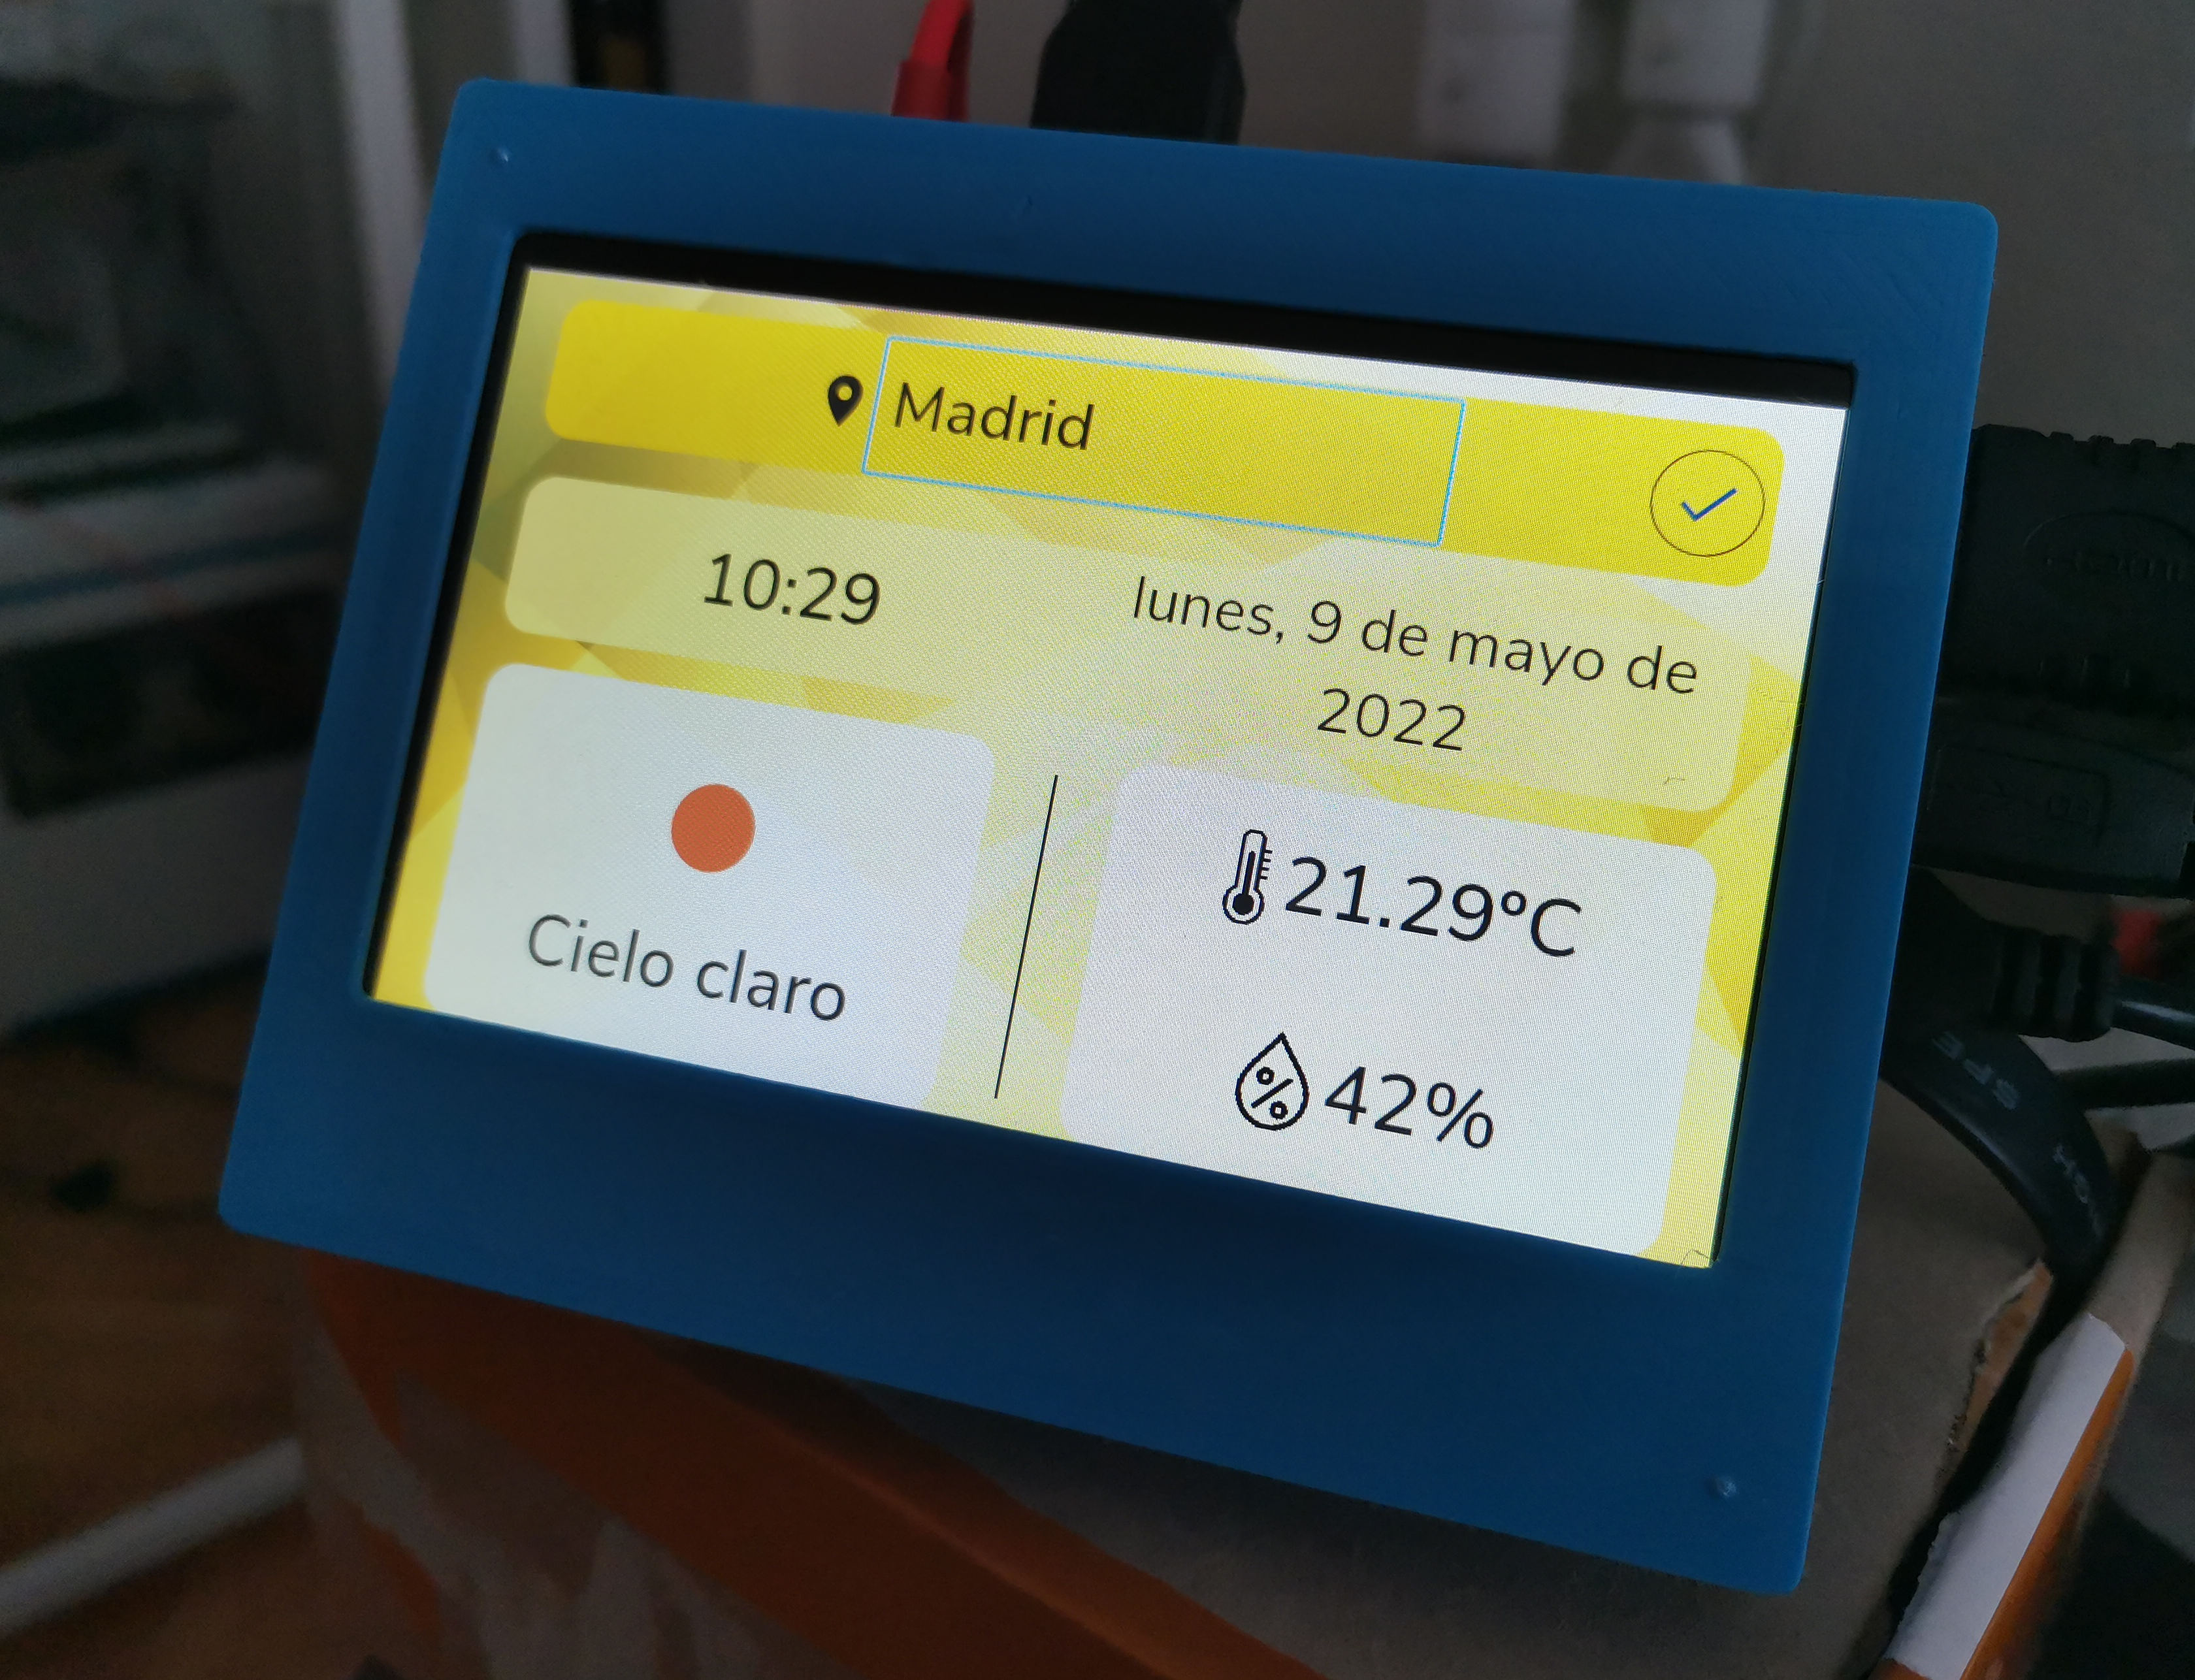
\includegraphics[width=0.70\linewidth]{imgs/app1}
	\caption[Rpi Weather]{Rpi Weather.}
	\label{img:rpi-weather-app}
\end{figure}

\section{Sistema Operativo FlutterPi.}\label{sec:flutterpi}

\paragraph{}El sistema operativo Flutter Pi es un sistema basado en el kernel de Linux,
generado con Yocto con las siguientes características principales:

\begin{itemize}
    \item Compatible con Raspberry Pi (ARMv7) de 32 bits.
    \item Incluye el motor embebido de Flutter.
    \item Incluye drivers gráficos de Vulkan con simulación de switfshaders.
    \item Incluye la configuración de una red Wi-Fi.
    \item Compatibilidad con pantalla LCD 5" táctil a través de HDMI.
    \item Servicio de arranque automático de la aplicación Flutter configurada.
    \item Servicio de levantamiento de interfaz Wi-Fi y conexión automática con
    punto de acceso configurado.
\end{itemize}

\section{El Prototipo.}\label{sec:prototipo}

\paragraph{}El aspecto exterior del prototipo, está caracterizado por su carcasa impresa
en 3D. La carcasa está divida modularmente en tres partes diferentes: la carcasa de la
pantalla LCD 5", la carcasa de la Raspberry Pi 3B+ y el soporte inclinado. Quiero
agradecer al usuario \href{https://www.thingiverse.com/thing:3444545}{ywabiko} de
Thingiverse su tiempo y dedicación en diseñar el modelo.

\paragraph{}El sistema en funcionamiento con la pantalla y la aplicación corriendo
tiene un cosumo eléctrico de 2,8-3,8 vatios a la hora, lo cuál es menos que una bombilla
led. Podríamos dejar el sistema corriendo siempre sin que represente un cambio significativo
en la factura de la luz. Podríamos utilizar una fuente de alimentación USB para alimentar
el sistema y sólo requeriría de una corriente máxima de 1 amperio.

\begin{figure}[H]
	\centering
	\subfigure[Trasera del prototipo]{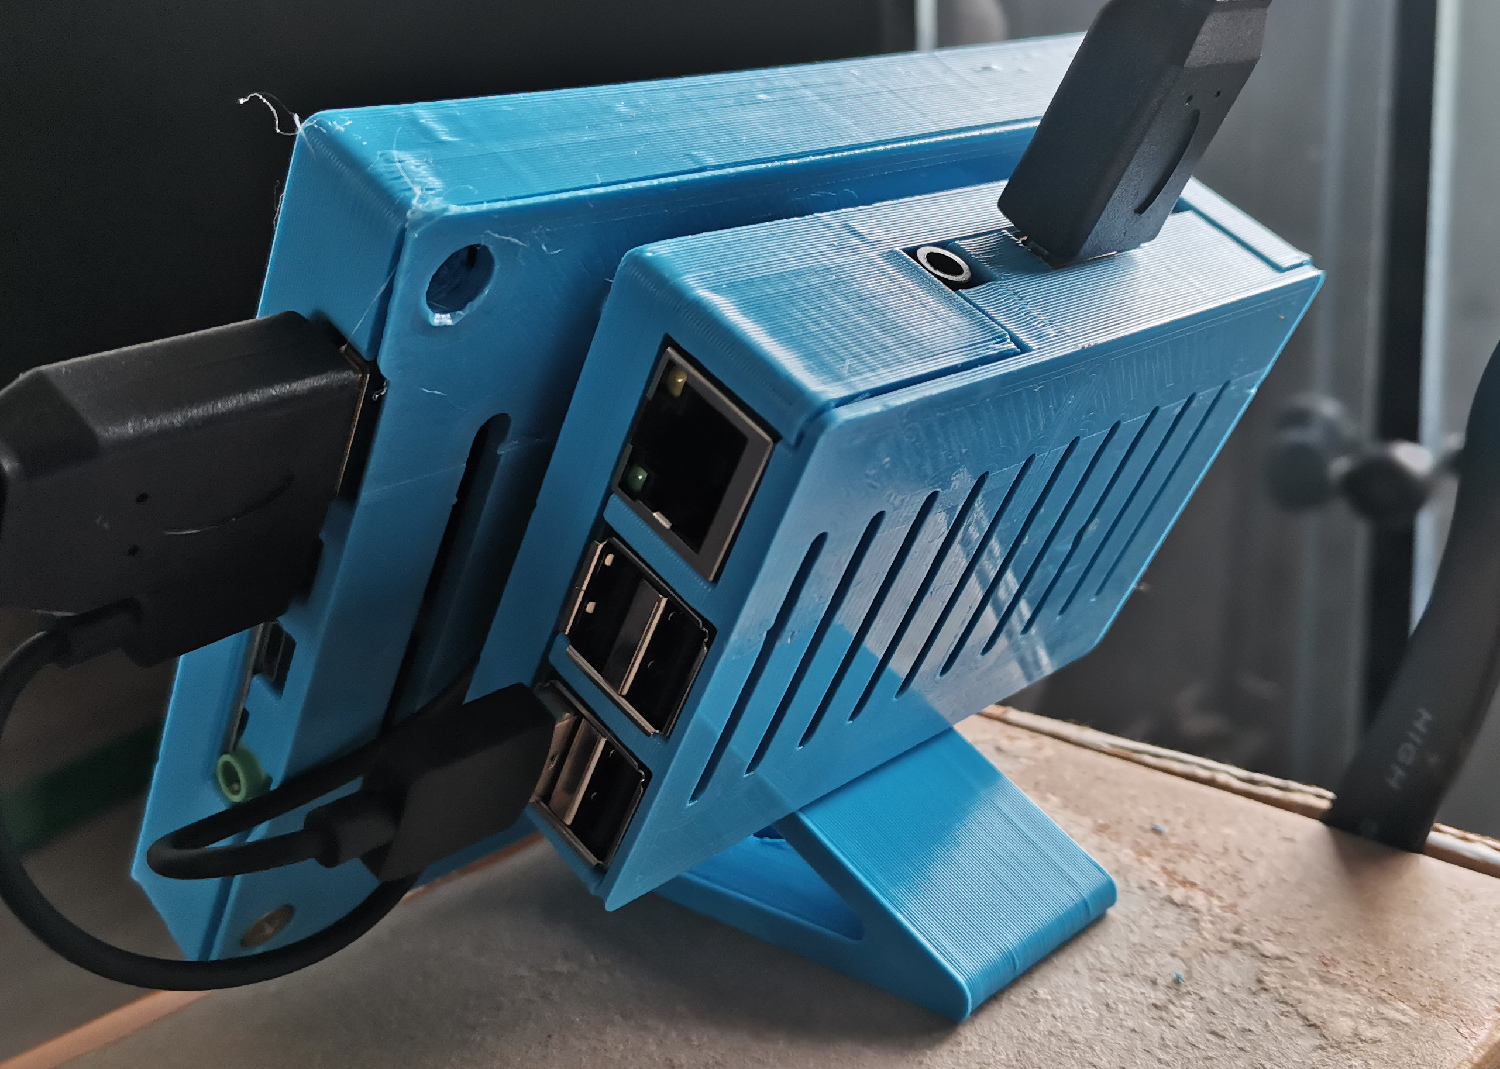
\includegraphics[width=0.4\linewidth]{imgs/proto-back1}}
    \subfigure[Trasera del prototipo]{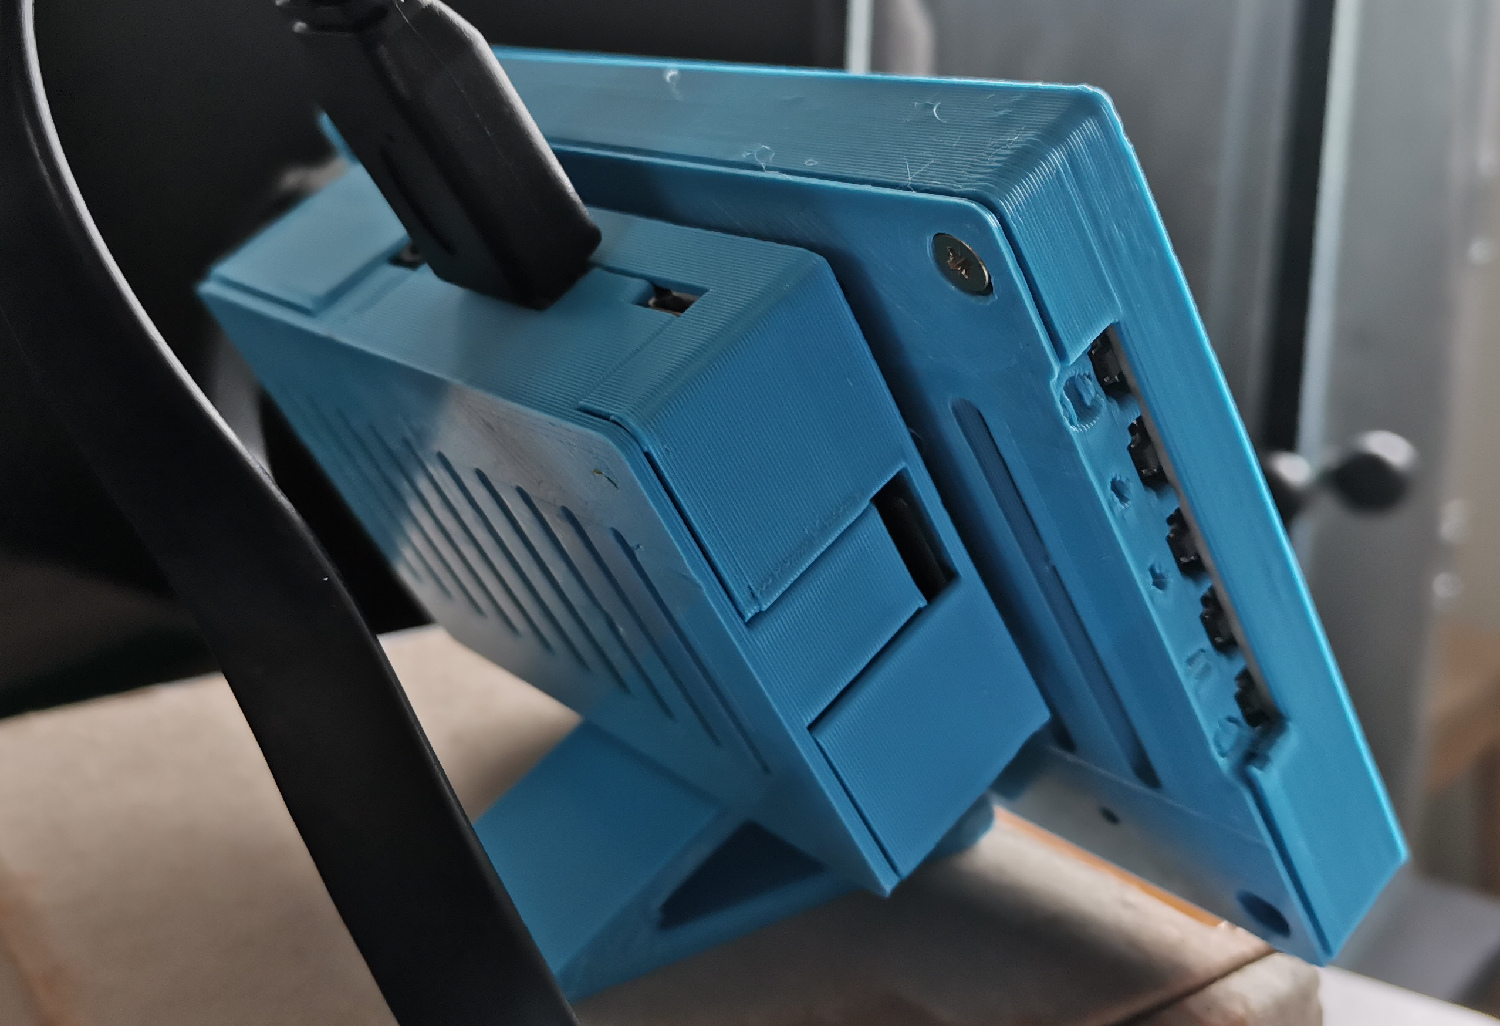
\includegraphics[width=0.4\linewidth]{imgs/proto-back2}}
    \subfigure[Frontal del prototipo]{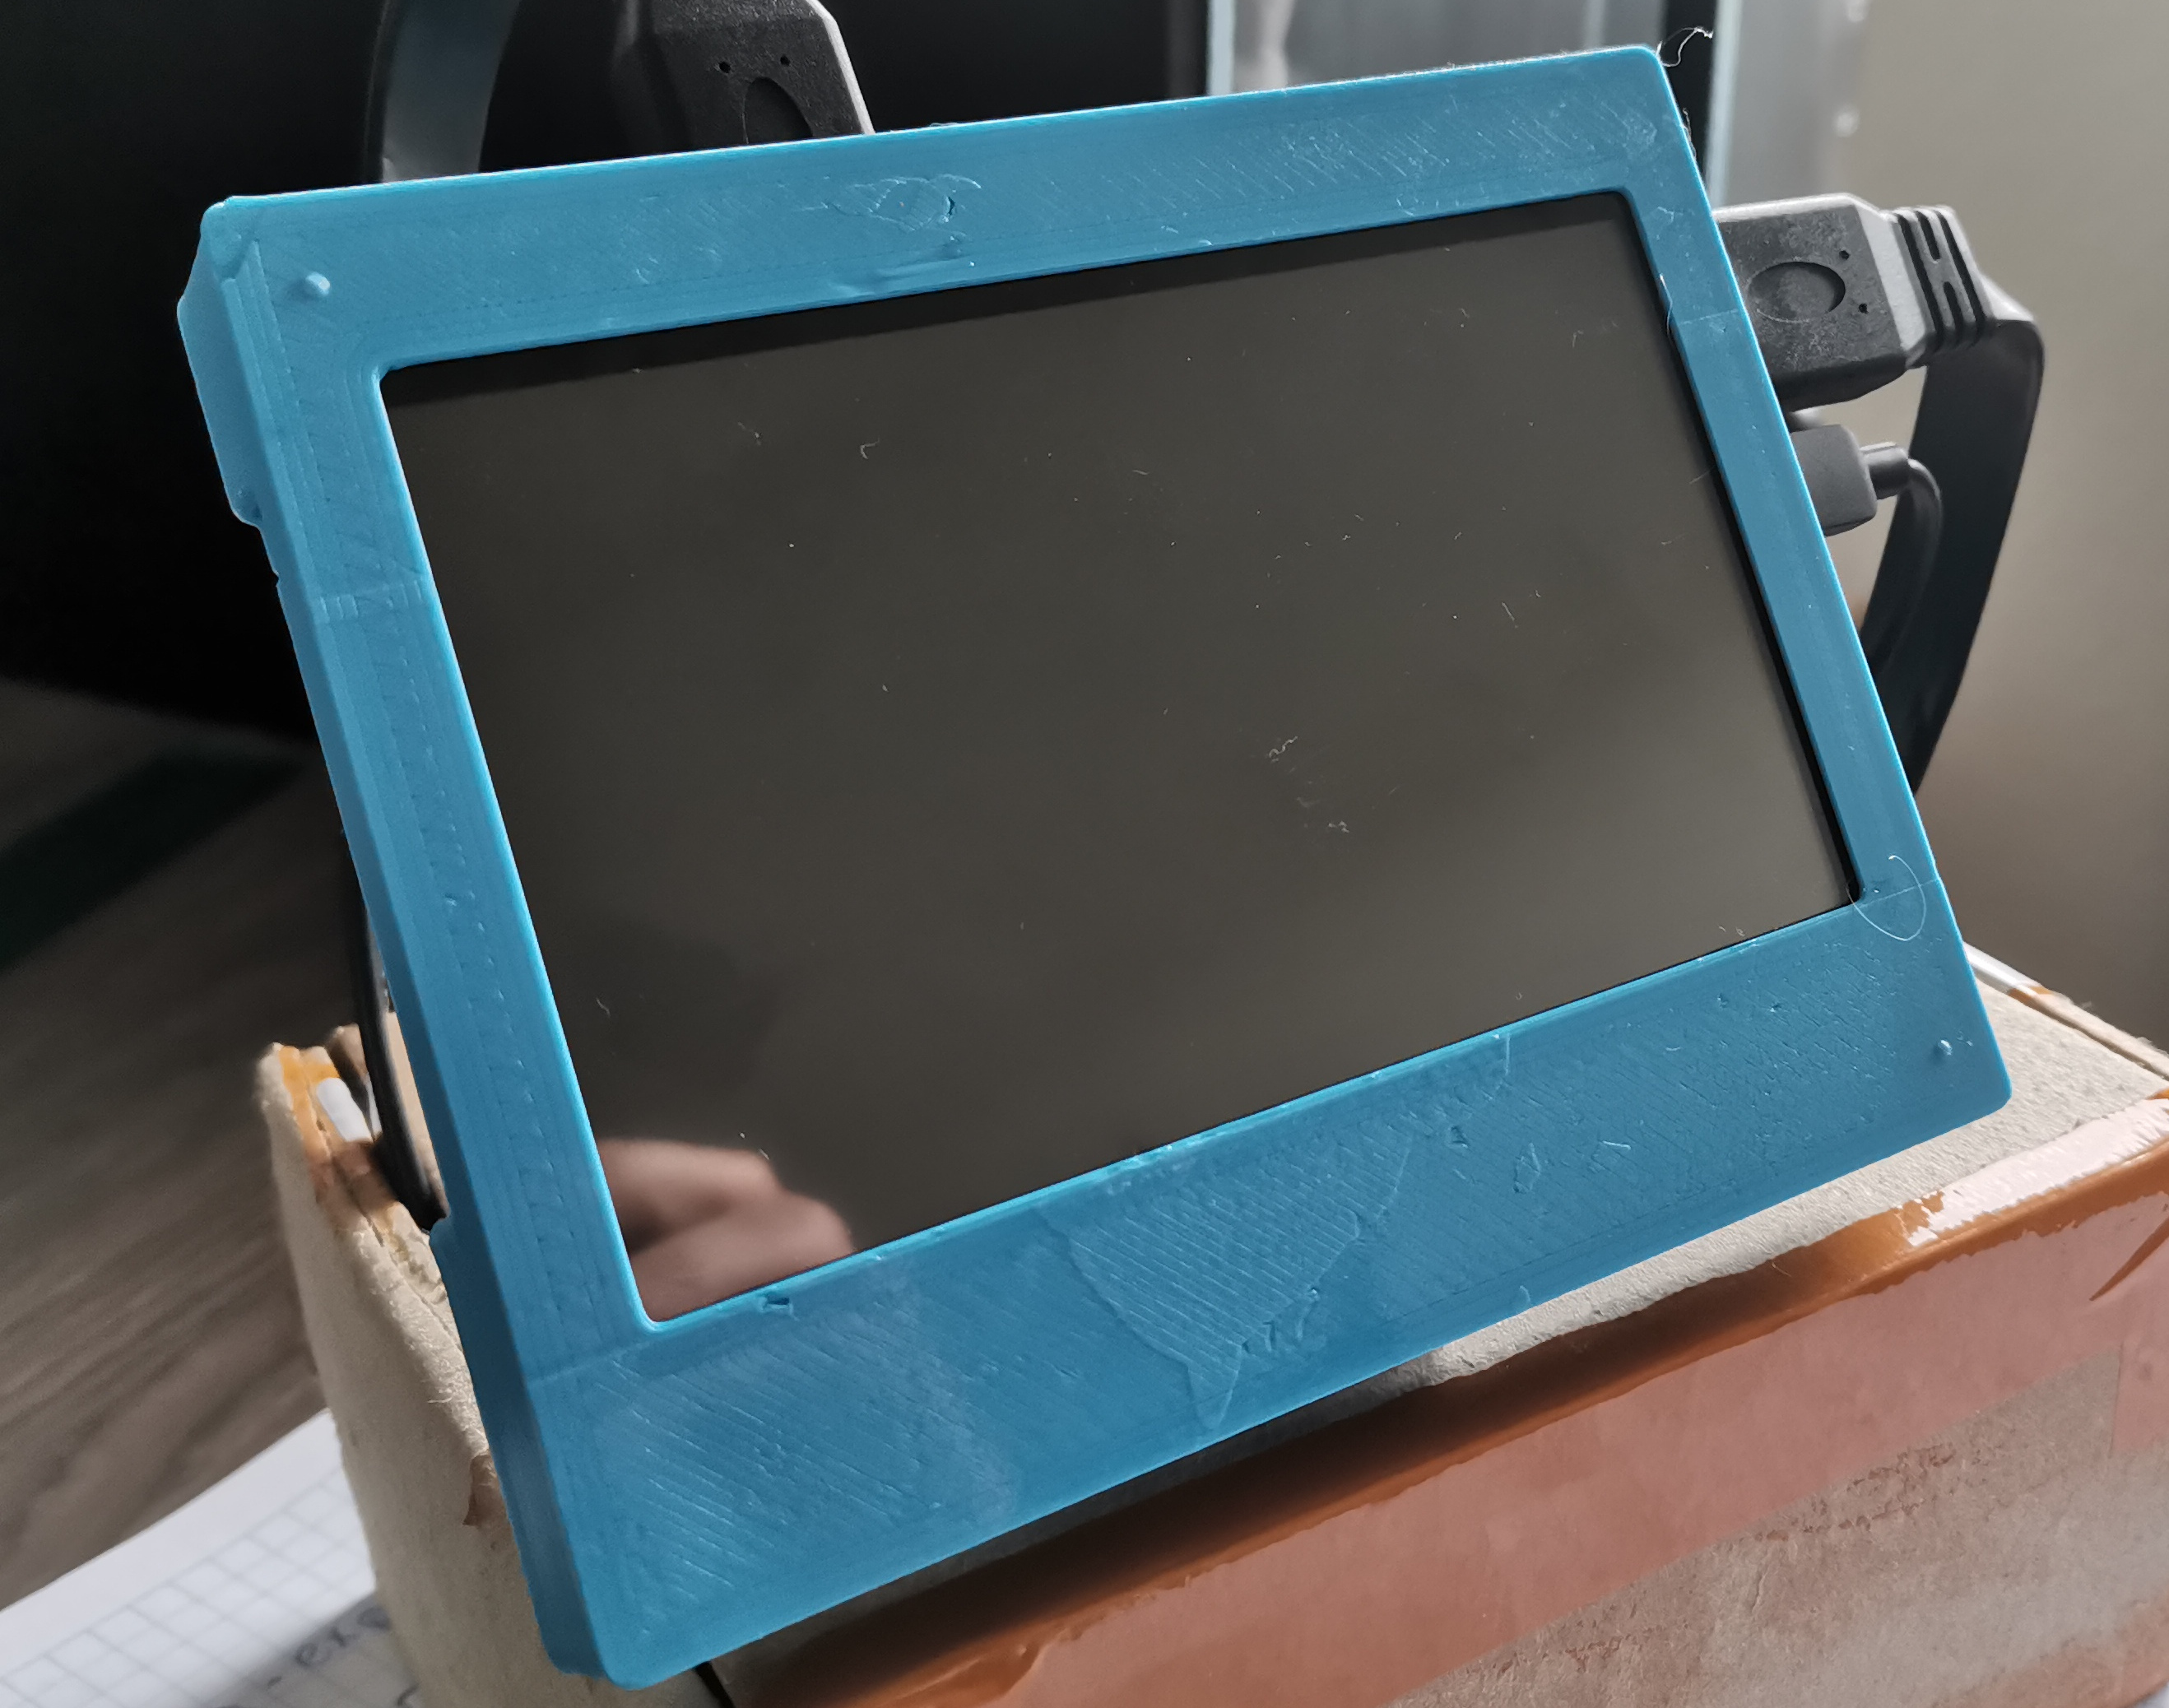
\includegraphics[width=0.4\linewidth]{imgs/proto-front}}
	\caption[Prototipo]{Diferentes vistas del prototipo.}
	\label{img:proto-views}
\end{figure}

%las referencias a artículos se ponen con \cite,
%las referencias a glosario \gls,
%y las referencias a ecuaciones \eqref
%las referencias a imgenes, tablas o figuras o secciones
% se ponen con \ref (sólo número) o con \hyperref[sec:X]{text}

\chapter{Gestión del proyecto}\label{sec:gestion}

En este capítulo se describe la gestión del proyecto: ciclo de vida, planificación,
presupuesto, etc.

\section{Ciclo de vida}


\section{Planificación}

\paragraph{}A continuación se muestra una planificacin por fases.

\subsection{Fase 1. Blabla}

\subsection{Fase 2. Blabla}

\subsection{Fase 3. Blabla}

\section{Presupuesto}

\subsection{Personal}

\paragraph{} Blabla

%\begin{table}[hbt]
%	\label{t:recursoshumanos}
%	\centering
%	\begin{tabular}{|c|c|c|c|}
%		\hline
%		\textbf{Mes} & \textbf{Das lab. empleados} & \textbf{Horas de Media [h/da]} & \textbf{Total mes [h]} \\
%		\hline
%		Febrero & 10 & 5 & 50 \\
%		\hline
%		\textbf{Total} &  &  & 714 \\
%		\hline
%	\end{tabular}
%	\caption{Desglose de horas dedicadas.}
%\end{table}

\subsection{Material}

\paragraph{}Los materiales utilizados son una Raspberry Pi rev.3 y su tarjeta microSD.

\subsection{Resumen de costes}

%\begin{table}[hbt]
%	\label{t:resumencostes}
%	\centering
%	\begin{tabular}{|c|c|c|c|}
%		\hline
%		\textbf{Producto} & \textbf{Coste unidad} & \textbf{Cantidad} & \textbf{Subtotal} \\
%		\hline
%		Rbpi rev.3 & 37 & 1 & 37 \\
%		\hline
%		microSD & 10 & 1 & 10 \\
%		\hline
%		\textbf{Total} &  &  & 47 \\
%		\hline
%	\end{tabular}
%\end{table}
\chapter{Conclusiones}\label{sec:conclusiones}

\paragraph{}Tras haber presentado los resultados del proyecto, vamos a terminar extrayendo
los aprendizajes y conclusiones más importantes.

\section{Cumplimiento de Objetivos principales}

\paragraph{}Blabla

\section{Cumplimiento de Objetivos secundarios}

\paragraph{}Blabla

\section{Aprendizajes}

\paragraph{}Blabla

\section{Continuación del desarrollo}

\paragraph{}Blabla

%las referencias a artculos se ponen con \cite,
%las referencias a imgenes \ref,
%las referencias a glosario \gls,
%y las referencias a ecuaciones \eqref

\backmatter
%genera doble hoja en blanco
\cleardoublepage

%estilo de bibliografía: plana, alfa...
\bibliographystyle{apalike}
%apartado de bibliografía
\addcontentsline{toc}{chapter}{Bibliografía}
%se incluye la bibliografía. Archivo de tipo .bib (bibtex)
\bibliography{bib/bibliografia}

%fin del documento
\end{document}